\documentclass[12pt]{article}
\usepackage{xepersian}
\settextfont{XB Niloofar}
\setlatintextfont{Times New Roman}
\setlength{\parskip}{1em}

\usepackage{amsmath}
\usepackage{xcolor}
\usepackage{titlesec}
\usepackage{graphicx}
\usepackage{subcaption}
\usepackage{tikz}
\usetikzlibrary{positioning, arrows.meta, shapes.geometric, fit, calc}

\tikzset{
    block/.style={rectangle, draw, thick, minimum height=1.1cm, minimum width=2.6cm, align=center, fill=gray!8},
    io/.style={rectangle, draw, thick, minimum height=0.8cm, minimum width=1.6cm, align=center, fill=blue!6},
    sig/.style={-{Latex[length=2mm]}, thick},
}

\begin{document}

% ---------- Title page ----------
\begin{center}
    \Large \textbf{گزارش کار آزمایشگاه مدار منطقی} \\[0.5em]
    \textbf{آزمایش دوم}
\end{center}

\vspace{2em}

\begin{center}
    دانشجویان:\\
    امیرحسین قرقانی -- 404106225\\
    محمد رجایی -- 404105842
\end{center}

\newpage

% ---------- Section 1 ----------
\section{شرح و هدف آزمایش}

هدف از این آزمایش، آشنایی کامل با نحوه کارکرد انواع شیفت‌رجیسترها و کاربردهای آن‌ها در ذخیره‌سازی و جابه‌جایی داده‌های دودویی است. این آزمایش در دو محیط شبیه‌سازی Proteus و Logisim و طی چهار مرحلهٔ اصلی زیر انجام می‌شود:

\begin{itemize}
    \item طراحی و ساخت یک شیفت‌رجیستر یک‌طرفهٔ ۴ بیتی با قابلیت بارگذاری موازی، با استفاده از فلیپ‌فلاپ‌های D و گیت‌های پایه.
    \item تبدیل مدار فوق به یک شیفت‌رجیستر دوطرفه که بر اساس سیگنال کنترلی $Mode$ می‌تواند به راست یا به چپ شیفت دهد.
    \item پیاده‌سازی همان عملکرد با استفاده از تراشهٔ آمادهٔ 7495 و مقایسهٔ آن با طراحی گسسته.
    \item طراحی یک مدار ترکیبی برای تشخیص رشته‌های خاص در خروجی شیفت‌رجیستر.
\end{itemize}

در ادامهٔ گزارش، ابتدا روش طراحی انتخاب‌شده برای هر بخش توضیح داده می‌شود، سپس بلوک‌دیاگرام کلی هر مدار پیش از ورود به جزئیات سیم‌کشی ارائه می‌گردد و در نهایت روند پیاده‌سازی، شماتیک نهایی و نتایج تست کیس ها در هر دو محیط Proteus و Logisim گزارش می‌شود.

% ---------- Section 2 ----------
\section{بررسی و انتخاب روش طراحی}

پیش از ورود به جزئیات سیم‌کشی، روش طراحی انتخاب‌شده برای هر یک از چهار بخش آزمایش و دلیل انتخاب آن به‌طور خلاصه بیان می‌شود.

\paragraph{شیفت‌رجیستر یک‌طرفه با بارگذاری موازی.} برای انتخاب بین ورودی موازی ($A \ldots D$) و ورودی سری (خروجی فلیپ‌فلاپ مجاور) در هر مرحله، از ترکیب دو گیت AND و یک گیت OR به‌عنوان یک مالتی‌پلکسر ۲ به ۱ گسسته استفاده شده است؛  سیگنال $Mode$ به‌طور مستقیم AND ورودی موازی و پس از نات‌شدن AND ورودی سری را کنترل می‌کند، به همین دلیل فلیپ‌فلاپ نوع D برای ذخیرهٔ مقدار انتخاب‌شده در هر تیک کلاک به‌کار رفته است.

\paragraph{شیفت‌رجیستر دوطرفه.} به‌جای طراحی مدار کاملاً جدید، ساختار مرحلهٔ قبل حفظ و تنها مسیر ورودی سری هر مالتی‌پلکسر بازتعریف شده است: در حالت $Mode=1$ هر فلیپ‌فلاپ از خروجی فلیپ‌فلاپ پایین‌دست (شیفت به چپ) و در حالت $Mode=0$ از خروجی فلیپ‌فلاپ بالادست (شیفت به راست) گرفته می‌شود. این روش نسبت به طراحی از صفر، تغییرات کمتری در سیم‌کشی نیاز دارد و امکان مقایسهٔ مستقیم دو طراحی را فراهم می‌کند.

\paragraph{استفاده از تراشهٔ 7495.} در این بخش به‌جای پیاده‌سازی گسسته، از تراشهٔ آمادهٔ 7495 استفاده شده تا کاهش پیچیدگی سیم‌کشی و مزیت استفاده از IC‌های آماده در طراحی‌های عملی نشان داده شود. از آنجا که این تراشه در Logisim موجود نیست، معادل آن با استفاده از فلیپ‌فلاپ‌های D و دو کلاک مجزا برای دو مود ($SL$ و $SR$) بازسازی شده است.

\paragraph{تشخیص رشته.} برای طراحی مدار تشخیص‌دهندهٔ رشته‌های خواسته‌شده، با نوشتن جدول درستی بر اساس $Q_0$ تا $Q_3$ و ساده سازی معادله بولینی F ، یک مدار ترکیبی ساده (چند گیت AND و یک گیت OR\rl{)} طراحی شده که به‌صورت پیوسته خروجی شیفت‌رجیستر را بررسی کرده و به‌محض عبور یکی از رشته‌های هدف، خروجی $F$ را یک می‌کند.

% ---------- Section 3 ----------
\section{طراحی و ساخت شیفت رجیستر}

\subsection{طراحی در پروتئوس}

در بخش اول، باید مدار شیفت رجیستر را مطابق شماتیک قرار داده شده در دستور کار پیاده‌سازی کنیم. این مدار به این صورت کار می‌کند که در صورتی که $Mode = 1$ ورودی‌های A تا D وارد شیفت رجیستر می‌شوند و در غیر این صورت، با در نظر گرفتن A به عنوان MSB، یک شیفت به راست می‌دهد و بیت $S_{in}$ را به عنوان مقدار جدید وارد $Q_{A}$ می‌کند. شکل~\ref{fig:simple-shift-register}

پیش از ورود به جزئیات سیم‌کشی، بلوک‌دیاگرام کلی این مدار در شکل~\ref{fig:block-oneway} نشان داده شده است. همان‌طور که دیده می‌شود، هر مرحله از یک مالتی‌پلکسر ۲ به ۱ (کنترل‌شده با $Mode$) و یک فلیپ‌فلاپ D تشکیل شده و مراحل به‌صورت زنجیره‌ای به یکدیگر متصل‌اند. همانطور که اشاره شد در بخش قبل، منظور از مالتی پلکسر ترکیب دو گیت AND و یک گیت OR است که در پیاده سازی نهایی استفاده شده و هیچ جایی از خود قطعه مالتی‌پلکسر به طور مستقیم استفاده نشده است.

در نهایت پس از ساخت شیفت رجیستر، با قرار دادن $Mode = 1$ مقدار 1010 را ذخیره می‌کنیم. (شکل ~\ref{fig:1010-register-initial} و ~\ref{fig:1010-registered})


برای بخش بعدی، با قرار دادن $Mode = 0$، شیفت رجیستر را وارد حالت شیفت به راست می‌کنیم و یک شیفت رجیستر با قابلیت شیفت به راست می‌سازیم. (شکل ~\ref{fig:sin-steps-proteus})


سپس از ما خواسته شده شیفت رجیستر با بسته به مقدار $Mode$ تبدیل به یک شیفت رجیستر دو طرفه کنیم. در حالت $Mode = 1$ شیفت رجیستر ما بدون تغییر است پس باید حالت مربوط به مقدار 0 را دستکاری کنیم. در حالت مقدار صفر، مدار مقادیر جدید شیفت رجیستر را از ورودی‌های A تا D می‌خواند و وارد فلیپ فلاپ‌ها می‌کند. کافی است همانطور که خروجی هر فلیپ فلاپ با $Mode = 1$ قبل از ورودی فلیپ فلاپِ بیتِ با ارزش کمتر ``AND'' گرفته می‌شد ($Q_{i} \cdot Mode$)، حال با نات شده $Mode$، قبل از ورودی فلیپ فلاپِ بیتِ با ارزش بیشتر ``AND'' گرفته شود. (شکل ~\ref{fig:twoway-shift-proteus} تا ~\ref{fig:twoway_rightshift-example-proteus})

بلوک‌دیاگرام این مدار در شکل~\ref{fig:block-twoway} آمده است. تفاوت اصلی نسبت به شکل~\ref{fig:block-oneway} در این است که ورودی مالتی‌پلکسر هر مرحله دیگر از ورودی موازی مستقل، بلکه از خروجی فلیپ‌فلاپ همسایه (بالادست یا پایین‌دست) تأمین می‌شود و انتخاب جهت شیفت با $Mode$ کنترل می‌شود.

\clearpage

\begin{figure}[htbp]
	\centering
	\beginL
	\begin{tikzpicture}[node distance=0.5cm and 1.3cm]
		\node[io] (par) {\RL{ورودی‌های موازی}\\$A,B,C,D$};
		\node[io, below=of par] (sin) {$S_{in}$};
		\node[block, right=of par, minimum height=2.4cm, yshift=-0.9cm] (mux) {\RL{مالتی‌پلکسر ۲ به ۱}\\(AND-OR)\\\RL{کنترل:} $Mode$};
		\node[block, right=of mux, minimum height=2.4cm] (ff) {\RL{زنجیره چهار}\\\RL{فلیپ‌فلاپ} D\\$(Q_A \ldots Q_D)$};
		\node[io, right=of ff] (out) {\RL{خروجی‌ها}\\$Q_A, Q_B, Q_C, Q_D$};
		\node[io, below=1.1cm of mux] (mode) {$Mode$};
		\node[io, below=1.1cm of ff] (clk) {$CLK$};
		
		\draw[sig] (par.east) -- (par.east -| mux.west);
		\draw[sig] (sin.east) -- (sin.east -| mux.west);
		\draw[sig] (mux) -- (ff);
		\draw[sig] (ff) -- (out);
		\draw[sig] (mode) -- (mux);
		\draw[sig] (clk) -- (ff);
	\end{tikzpicture}
	\endL
	\caption{بلوک‌دیاگرام شیفت‌رجیستر یک‌طرفه با قابلیت بارگذاری موازی}
	\label{fig:block-oneway}
\end{figure}

\begin{figure}[htbp]
    \centering
    \beginL
    \begin{tikzpicture}[node distance=0.5cm and 1.3cm]
        \node[io] (sin) {$S_{in}$};
        \node[block, right=of sin, minimum height=2.4cm, yshift=0cm] (mux) {\RL{واحد کنترل جهت شیفت}\\\RL{کنترل:} $Mode$};
        \node[block, right=of mux, minimum height=2.4cm] (ff) {\RL{زنجیره چهار}\\\RL{فلیپ‌فلاپ} D \RL{دوطرفه}\\$(Q_A \ldots Q_D)$};
        \node[io, right=of ff] (out) {\RL{خروجی‌ها}\\$Q_A, Q_B, Q_C, Q_D$};
        \node[io, below=1.1cm of mux] (mode) {$Mode$};
        \node[io, below=1.1cm of ff] (clk) {$CLK$};

        \draw[sig] (sin) -- (mux);
        \draw[sig] (mux) -- (ff);
        \draw[sig] (ff) to[out=250, in=290] (mux);
        \node[font=\small] at ($(mux)!0.5!(ff)+(0,-1.75cm)$) {بازخورد‌بین‌مراحل‌مجاور};
        \draw[sig] (ff) -- (out);
        \draw[sig] (mode) -- (mux);
        \draw[sig] (clk) -- (ff);
    \end{tikzpicture}
    \endL
    \caption{بلوک‌دیاگرام شیفت‌رجیستر دوطرفه (بدون بارگذاری موازی)}
    \label{fig:block-twoway}
\end{figure}

\begin{figure}[htbp]
    \centering
    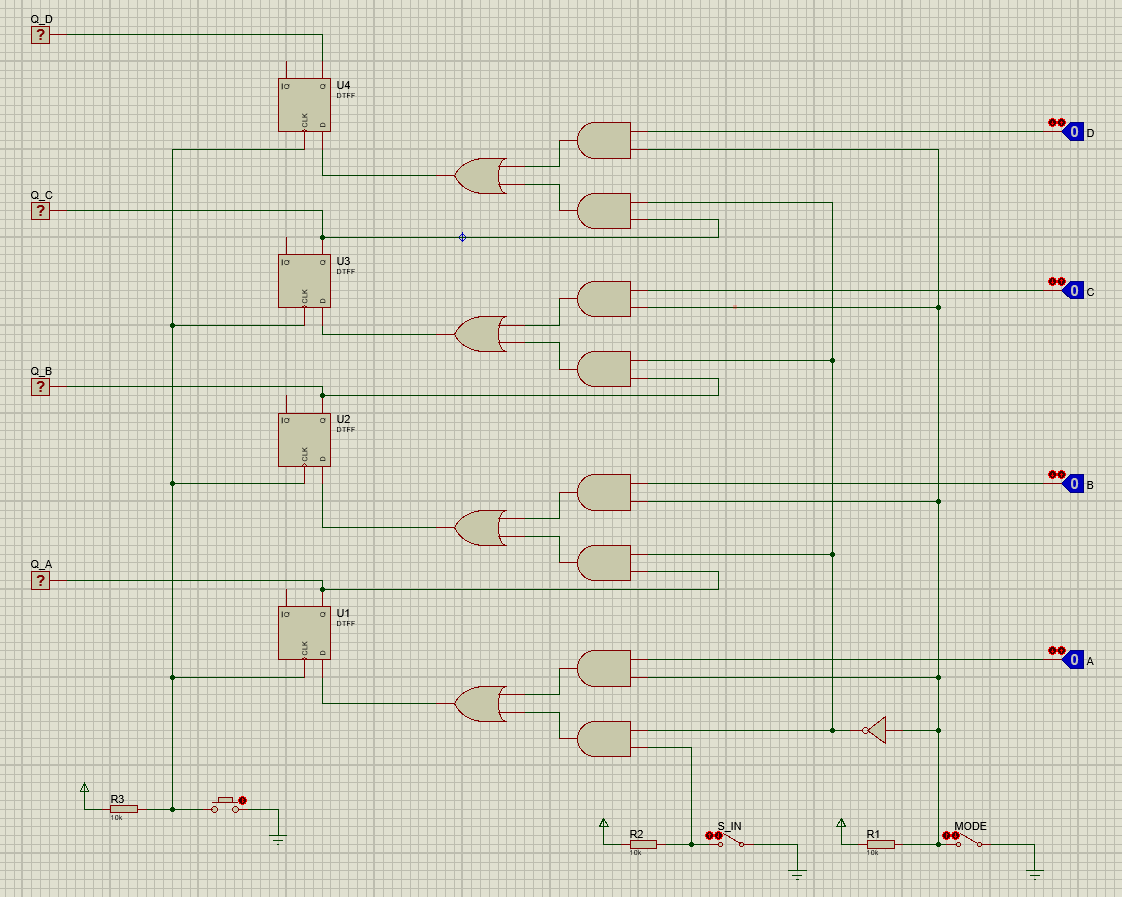
\includegraphics[width=1\textwidth]{Screenshot 2026-08-09 075038.png}
    \caption{پیاده سازی شیفت رجیستر یک طرفه اولیه در محیط پروتئوس}
    \label{fig:simple-shift-register}
\end{figure}

\newpage

\begin{figure}[htbp]
	\centering
	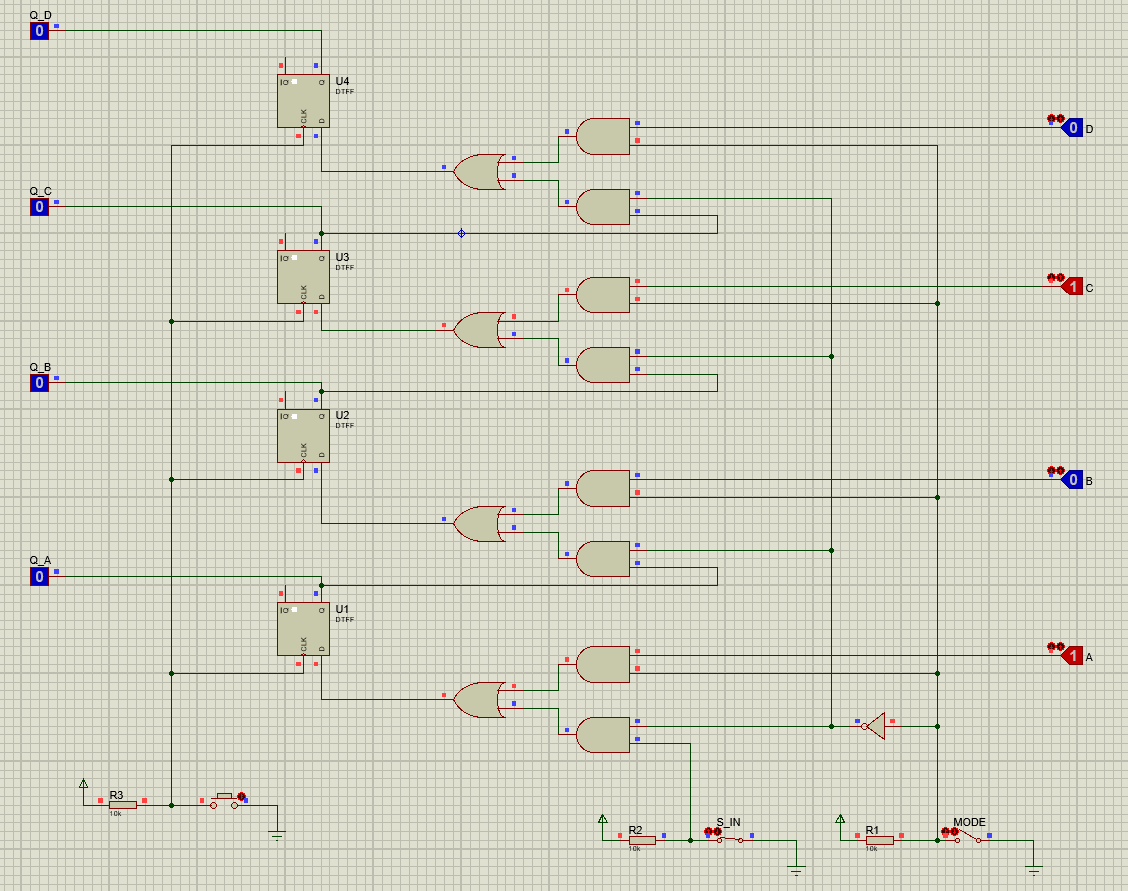
\includegraphics[width=1\textwidth]{Screenshot 2026-08-09 074832.png}
	\caption{وارد کردن مقدار 1010 به عنوان ورودی به مدار قبل از پیشبرد کلاک}
	\label{fig:1010-register-initial}
\end{figure}

\newpage

\begin{figure}[htbp]
	\centering
	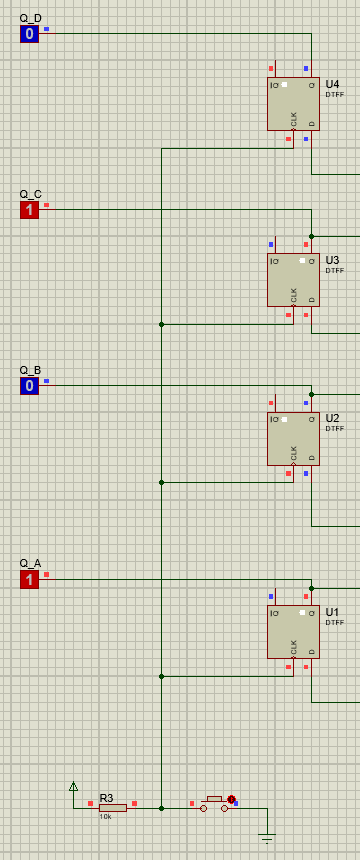
\includegraphics[width=0.55\textwidth]{Screenshot 2026-08-09 074913.png}
	\caption{خروجی و ذخیره 1010 بعد از یک تیک کلاک}
	\label{fig:1010-registered}
\end{figure}

\newpage


\begin{figure}[htbp]
	\centering
	\begin{subfigure}[b]{0.9\textwidth}
		\centering
		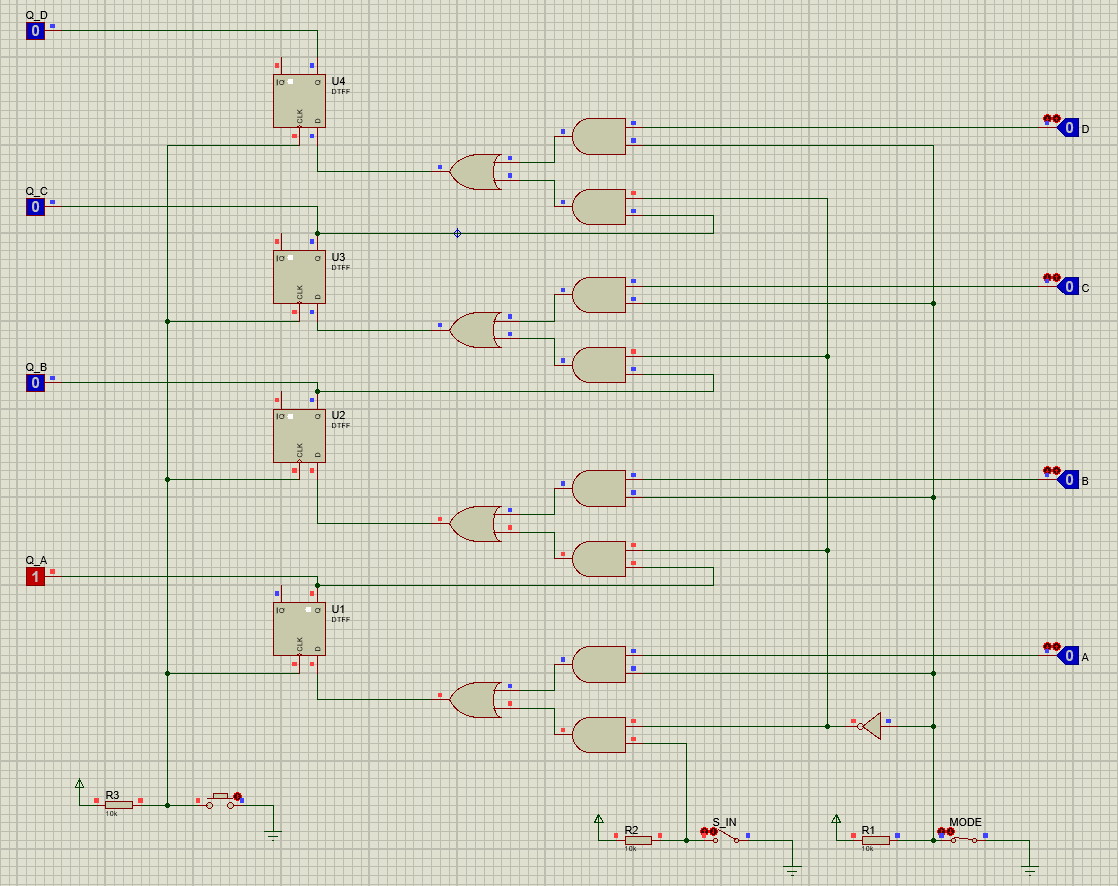
\includegraphics[height=0.33\textheight]{Screenshot 2026-08-09 075926.png}
		\caption{تیک اول}
	\end{subfigure}
	\hfill
	\begin{subfigure}[b]{0.9\textwidth}
		\centering
		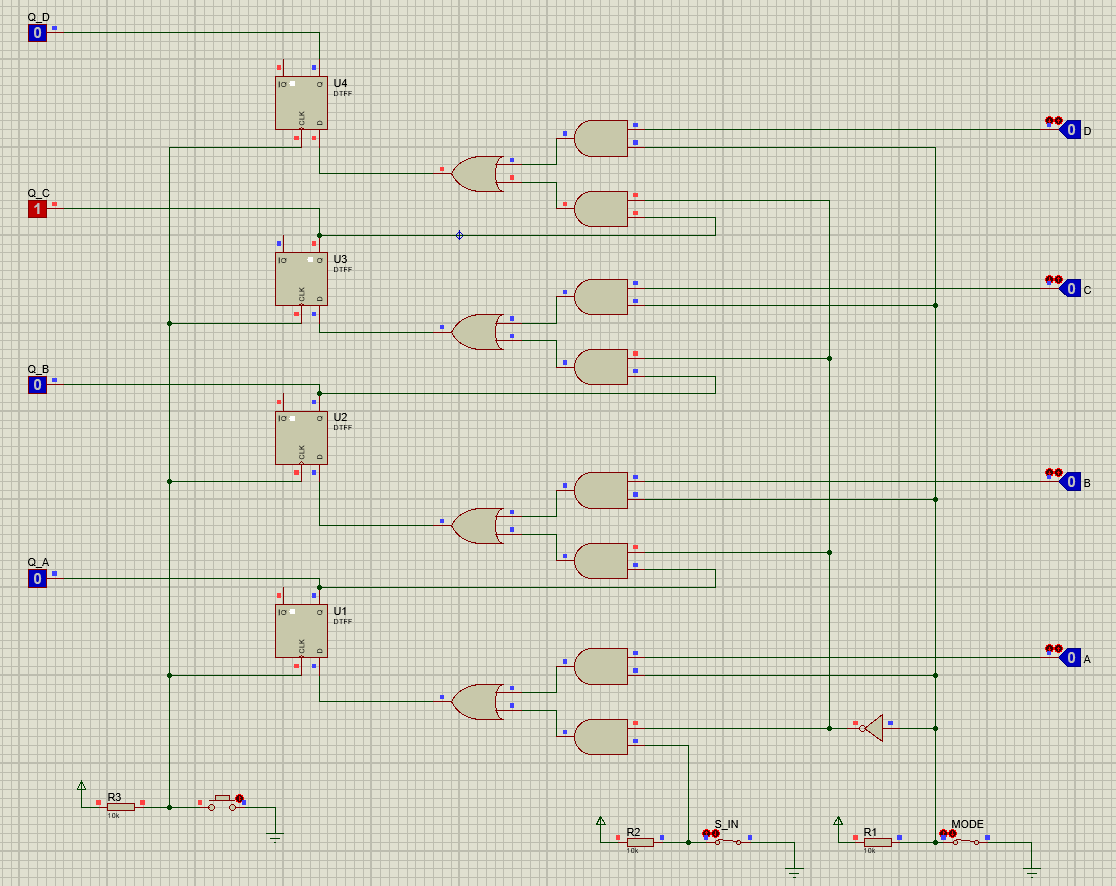
\includegraphics[height=0.33\textheight]{Screenshot 2026-08-09 075949.png}
		\caption{تیک دوم و سوم}
	\end{subfigure}
	\hfill
	\begin{subfigure}[b]{0.9\textwidth}
		\centering
		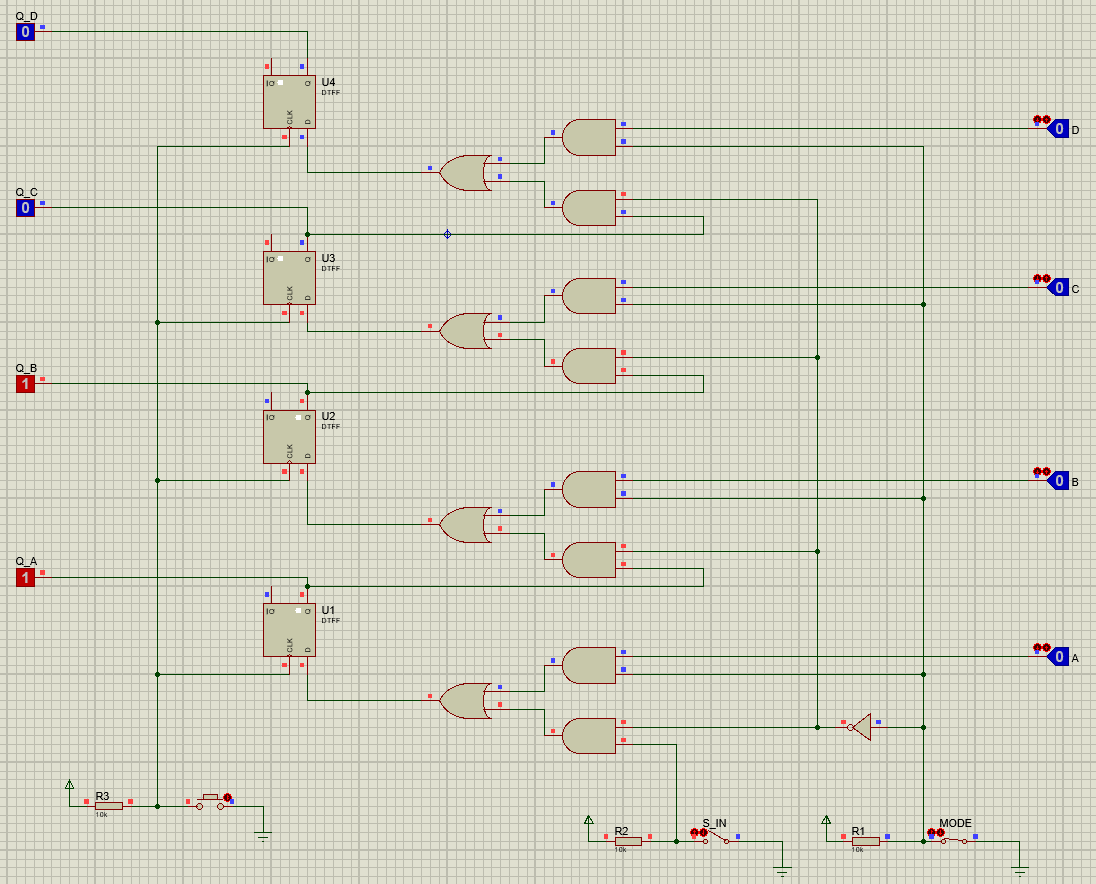
\includegraphics[height=0.33\textheight]{Screenshot 2026-08-09 080012.png}
		\caption{تیک چهارم و پنجم}
	\end{subfigure}
	\caption{نمایش قدم به قدم وارد شدن مقدار $S_{in}$ به ازای هر تیک}
	\label{fig:sin-steps-proteus}
\end{figure}


\newpage

\begin{figure}[htbp]
	\centering
	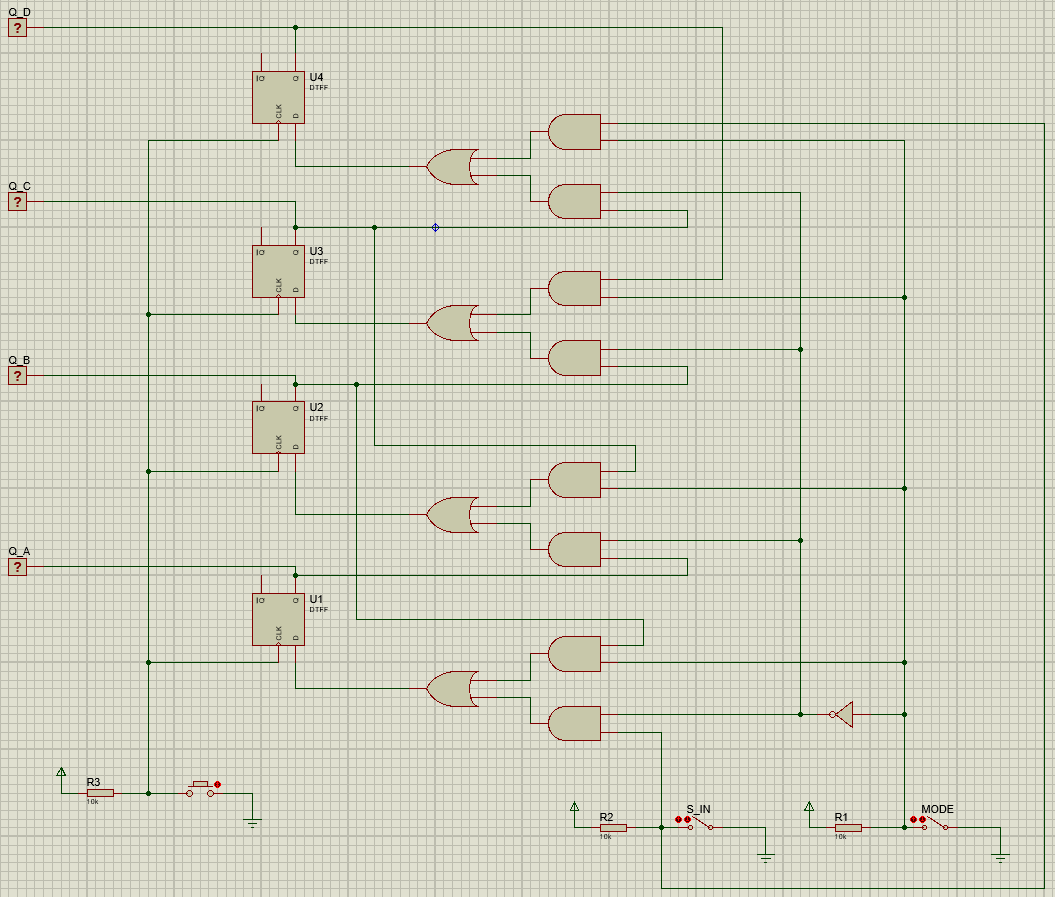
\includegraphics[width=1\textwidth, height=0.8\textheight]{Screenshot 2026-08-09 101442.png}
	\caption{پیاده سازی شیفت رجیستر با قابلیت شیفت دوطرفه در محیط پروتئوس}
	\label{fig:twoway-shift-proteus}
\end{figure}

\newpage

\begin{figure}[htbp]
	\centering
	\begin{subfigure}[b]{0.48\textwidth}
		\centering
		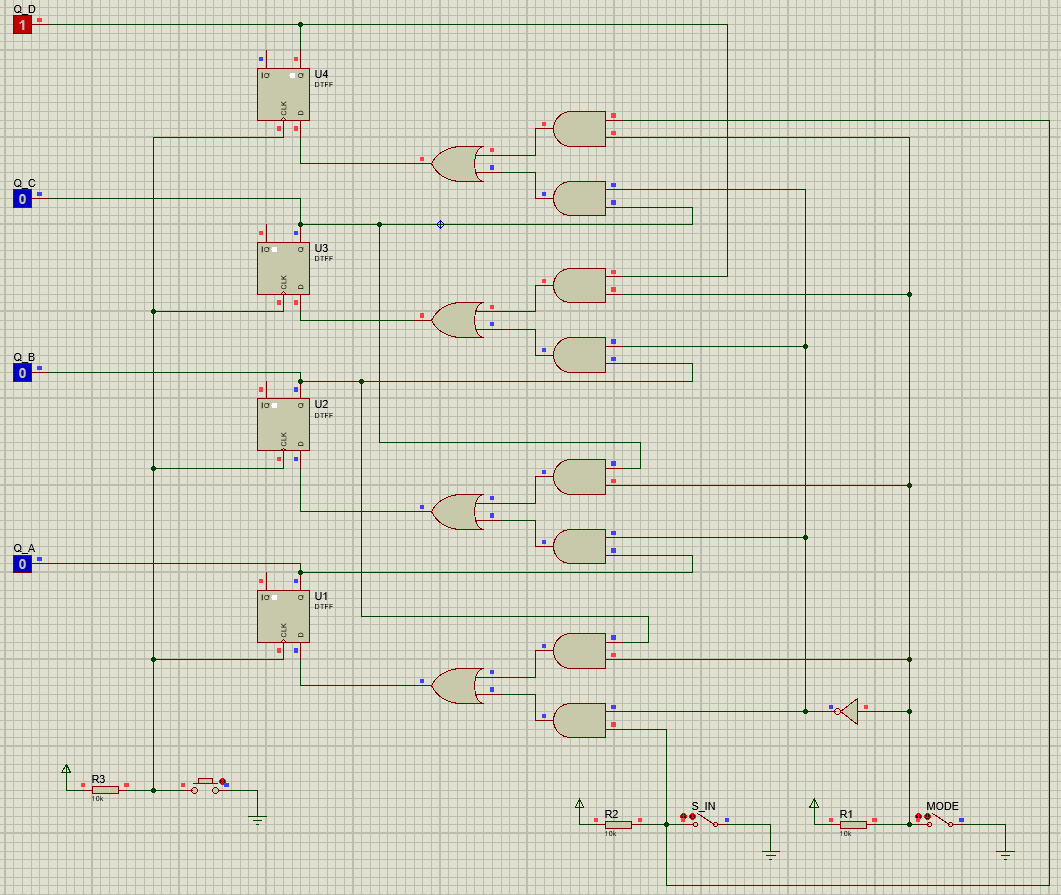
\includegraphics[width=\textwidth]{Screenshot 2026-08-09 101534.png}
		\caption{تیک اول}
		\label{fig:twoway-1}
	\end{subfigure}
	\hfill
	\begin{subfigure}[b]{0.48\textwidth}
		\centering
		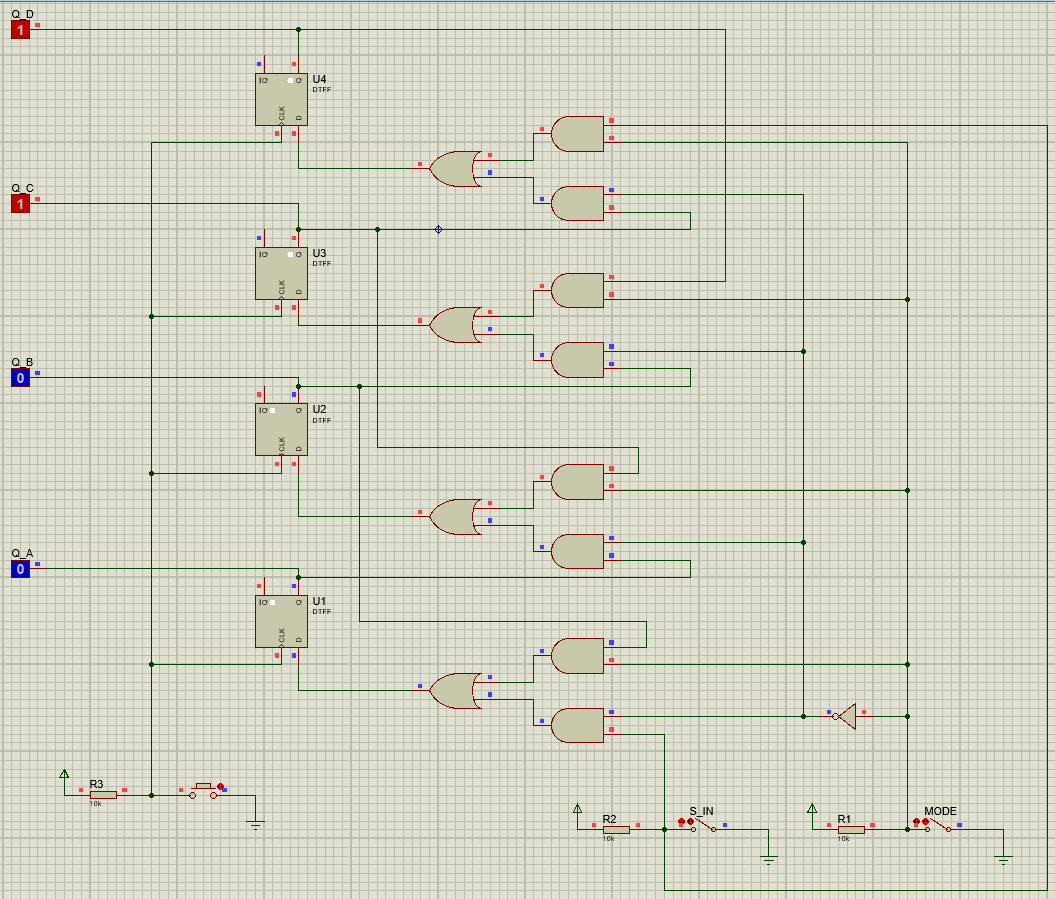
\includegraphics[width=\textwidth]{Screenshot 2026-08-09 101554.png}
		\caption{تیک دوم}
		\label{fig:twoway-2}
	\end{subfigure}
	
	\vspace{1em}
	
	\begin{subfigure}[b]{0.48\textwidth}
		\centering
		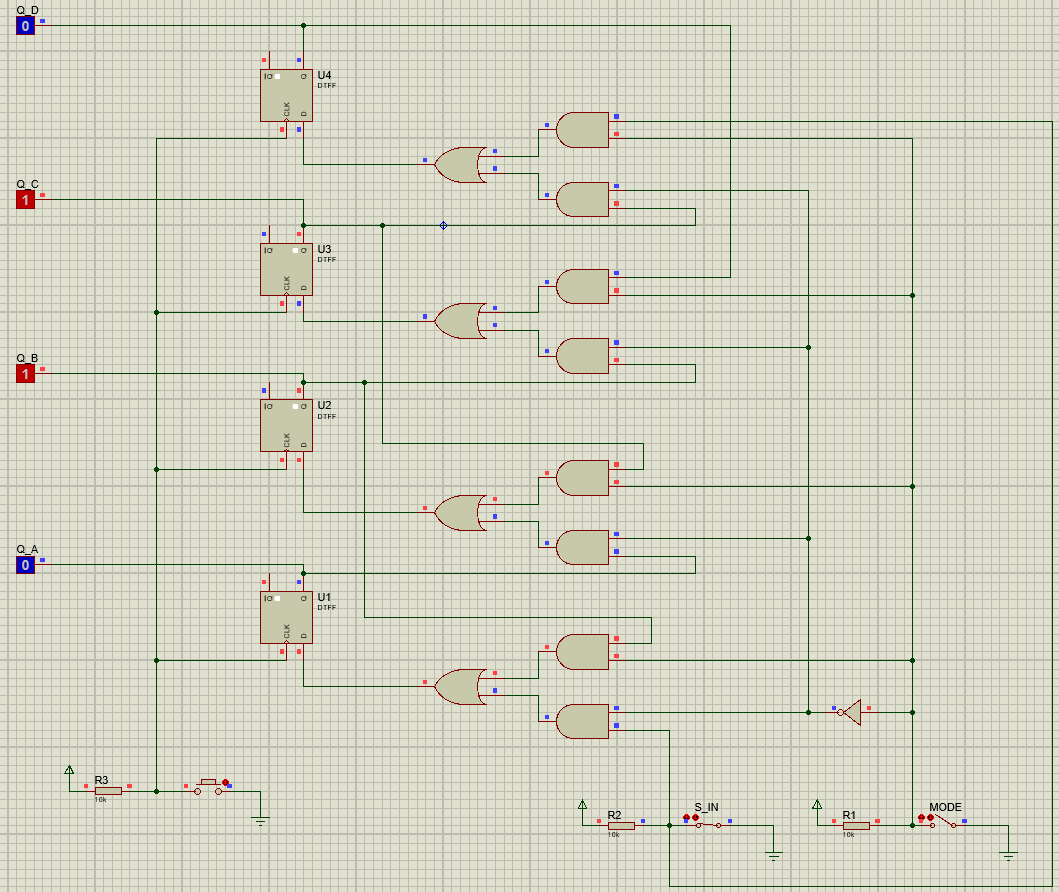
\includegraphics[width=\textwidth]{Screenshot 2026-08-09 101606.png}
		\caption{تیک سوم}
		\label{fig:twoway-3}
	\end{subfigure}
	\hfill
	\begin{subfigure}[b]{0.48\textwidth}
		\centering
		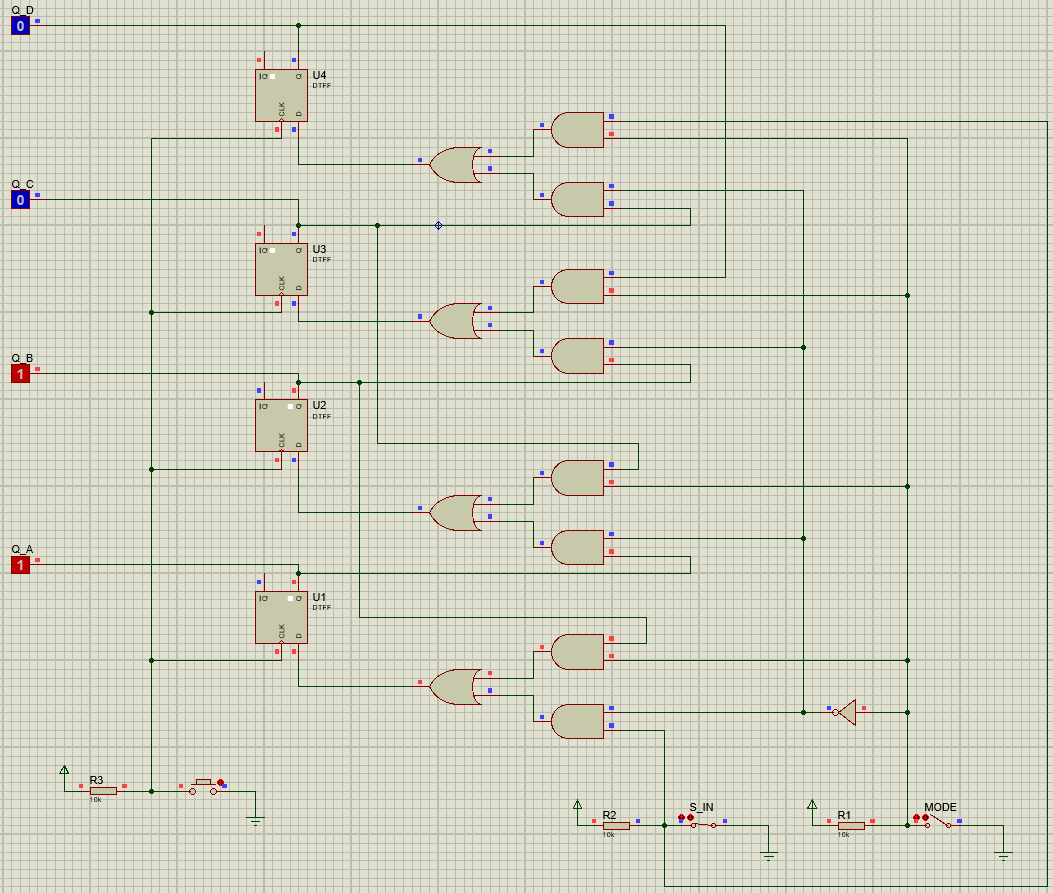
\includegraphics[width=\textwidth]{Screenshot 2026-08-09 101626.png}
		\caption{تیک چهارم}
		\label{fig:twoway-4}
	\end{subfigure}
	
	\caption{نمایش شیفت به سمت چپ در $Mode=1$}
	\label{fig:twoway-leftshift-example-proteus}
\end{figure}

\newpage

\begin{figure}[htbp]
	\centering
	\begin{subfigure}[b]{0.48\textwidth}
		\centering
		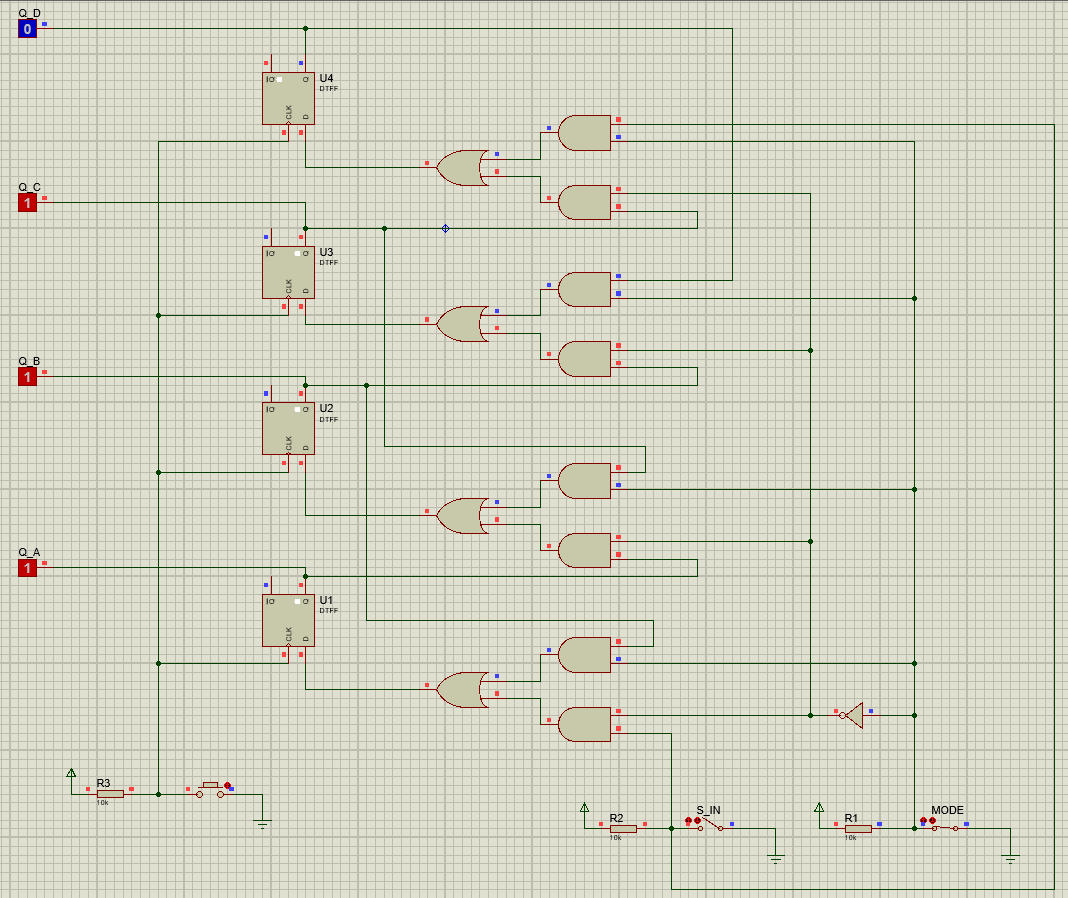
\includegraphics[width=\textwidth]{Screenshot 2026-08-09 101644.png}
		\caption{تیک اول}
		\label{fig:rightshift-1}
	\end{subfigure}
	\hfill
	\begin{subfigure}[b]{0.48\textwidth}
		\centering
		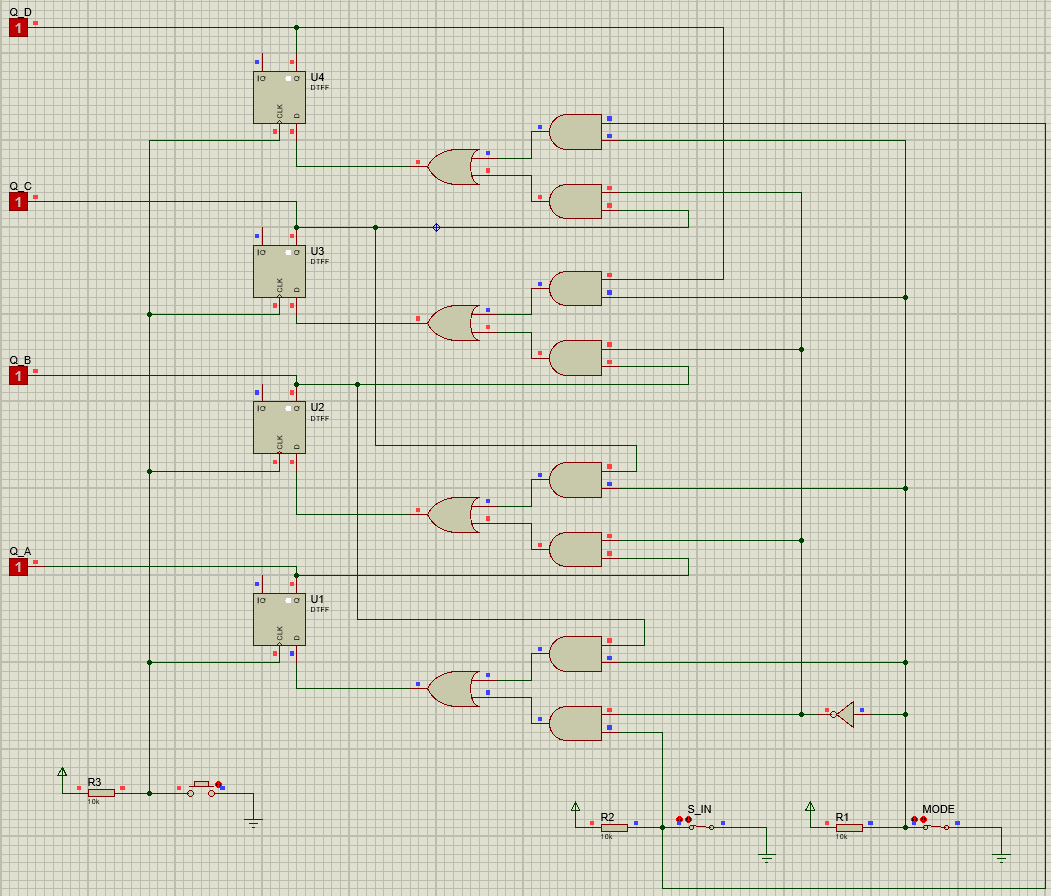
\includegraphics[width=\textwidth]{Screenshot 2026-08-09 101702.png}
		\caption{تیک دوم}
		\label{fig:rightshift-2}
	\end{subfigure}
	
	\vspace{1em}
	
	\begin{subfigure}[b]{0.48\textwidth}
		\centering
		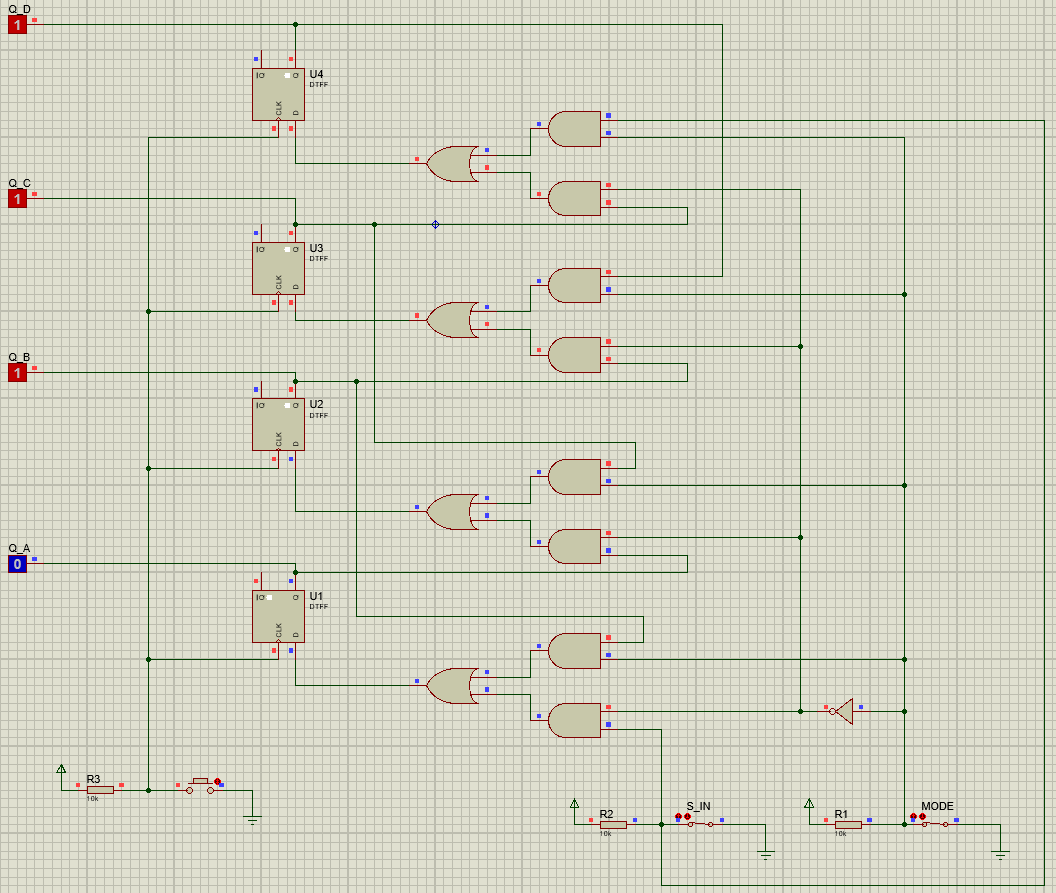
\includegraphics[width=\textwidth]{Screenshot 2026-08-09 101711.png}
		\caption{تیک سوم}
		\label{fig:rightshift-3}
	\end{subfigure}
	
	\caption{نمایش شیفت به سمت راست در $Mode=0$}
	\label{fig:twoway_rightshift-example-proteus}
\end{figure}

\clearpage

\subsection{طراحی در لاجیسیم}

پیاده سازی این بخش در لاجیسیم تفاوتی با پروتئوس ندارد و توضیحات قبلی اینجا هم صادق است.

\begin{figure}[htbp]
	\centering
	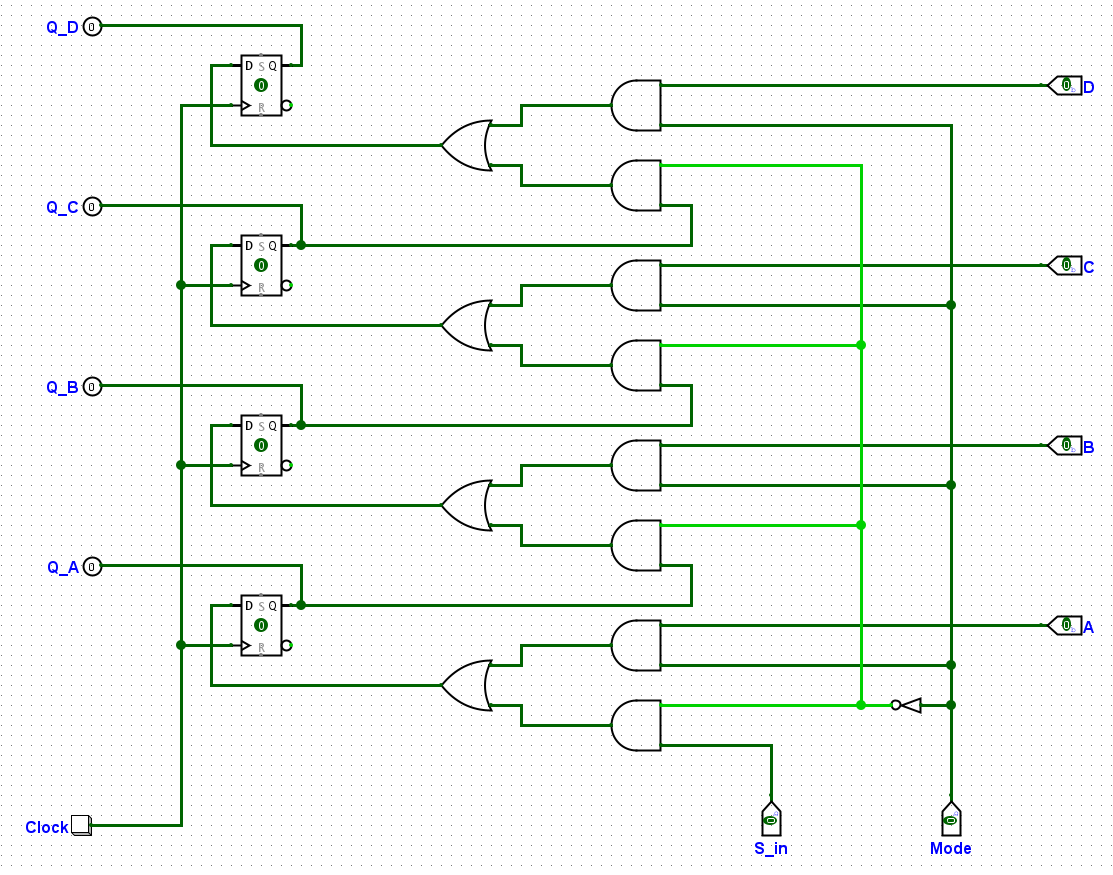
\includegraphics[width=1\textwidth]{Screenshot 2026-08-09 160023.png}
	\caption{پیاده سازی شیفت رجیستر خواسته شده اولیه در محیط لاجیسیم}
	\label{fig:simple-shift-register-logisim}
\end{figure}

\begin{figure}[htbp]
	\centering
	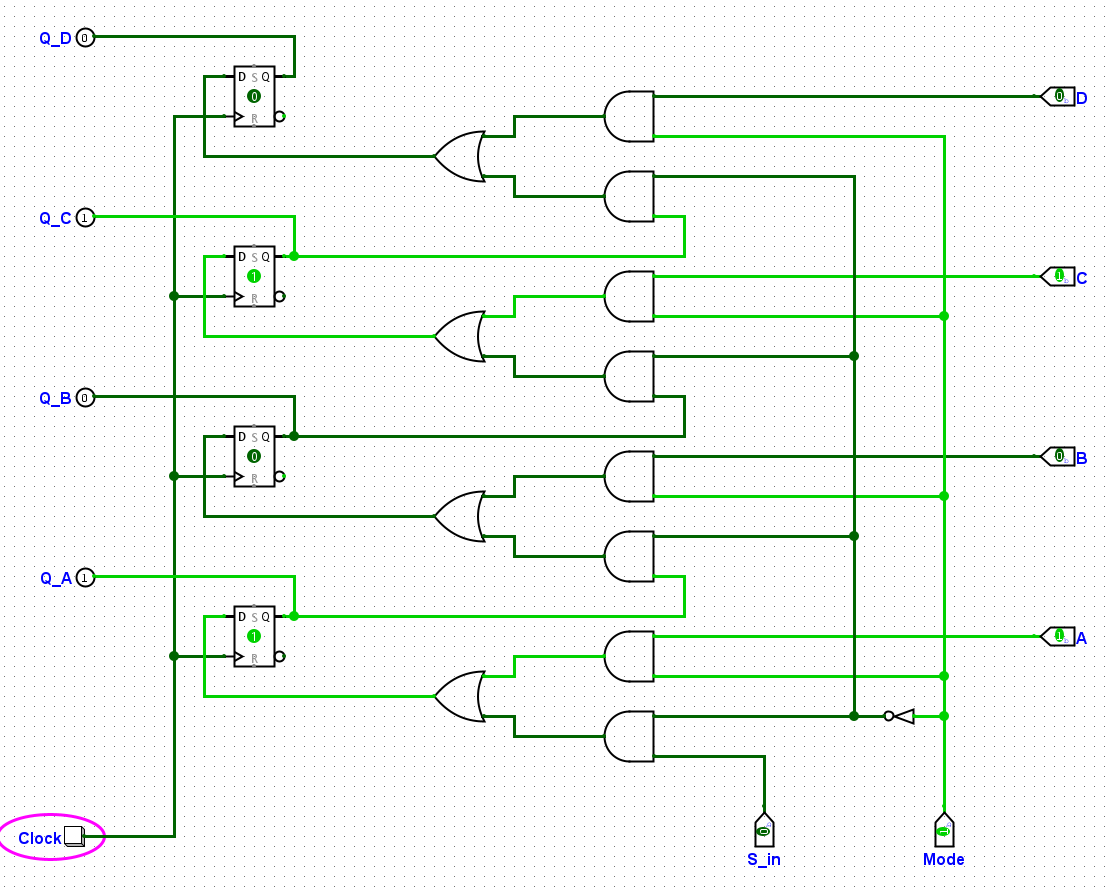
\includegraphics[width=1\textwidth]{Screenshot 2026-08-09 160347.png}
	\caption{ذخیره کردن مقدار 1010 در شیفت رجیستر در محیط لاجیسیم}
	\label{fig:1010-register-initial-logisim}
\end{figure}

\begin{figure}[htbp]
	\centering
	\begin{subfigure}[b]{0.48\textwidth}
		\centering
		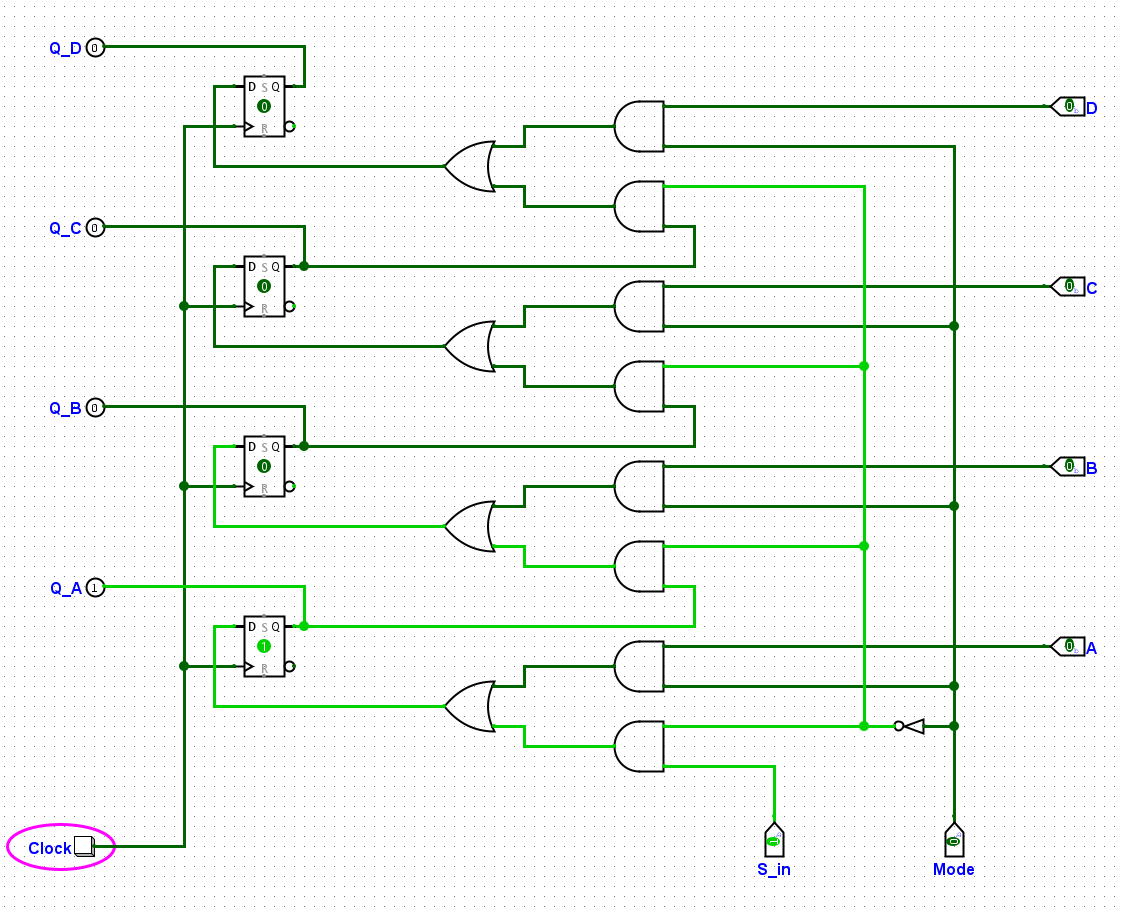
\includegraphics[width=\textwidth]{Screenshot 2026-08-09 160447.png}
		\caption{تیک اول}
		\label{fig:rightshift-1-logisim}
	\end{subfigure}
	\hfill
	\begin{subfigure}[b]{0.48\textwidth}
		\centering
		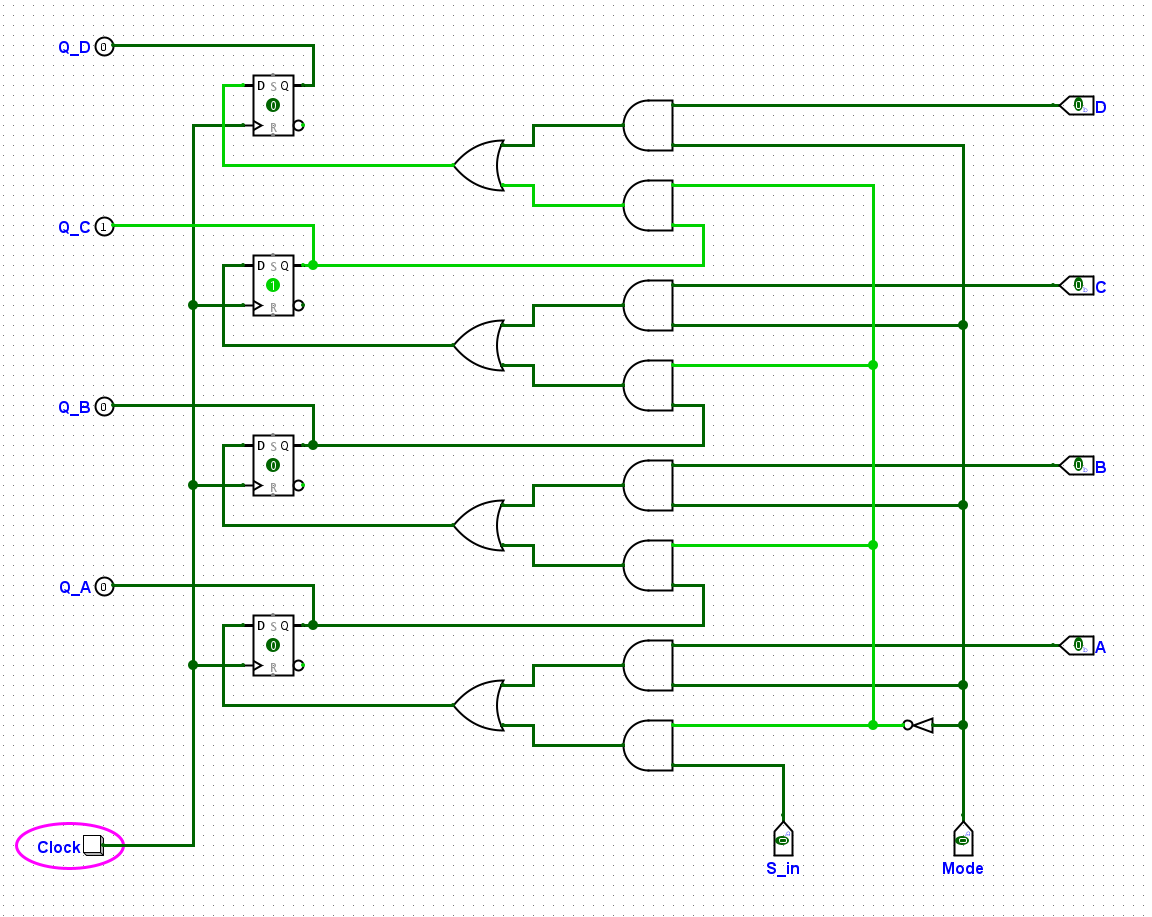
\includegraphics[width=\textwidth]{Screenshot 2026-08-09 160546.png}
		\caption{تیک دوم و سوم}
		\label{fig:rightshift-2-logisim}
	\end{subfigure}
	
	\vspace{1em}
	
	\begin{subfigure}[b]{0.48\textwidth}
		\centering
		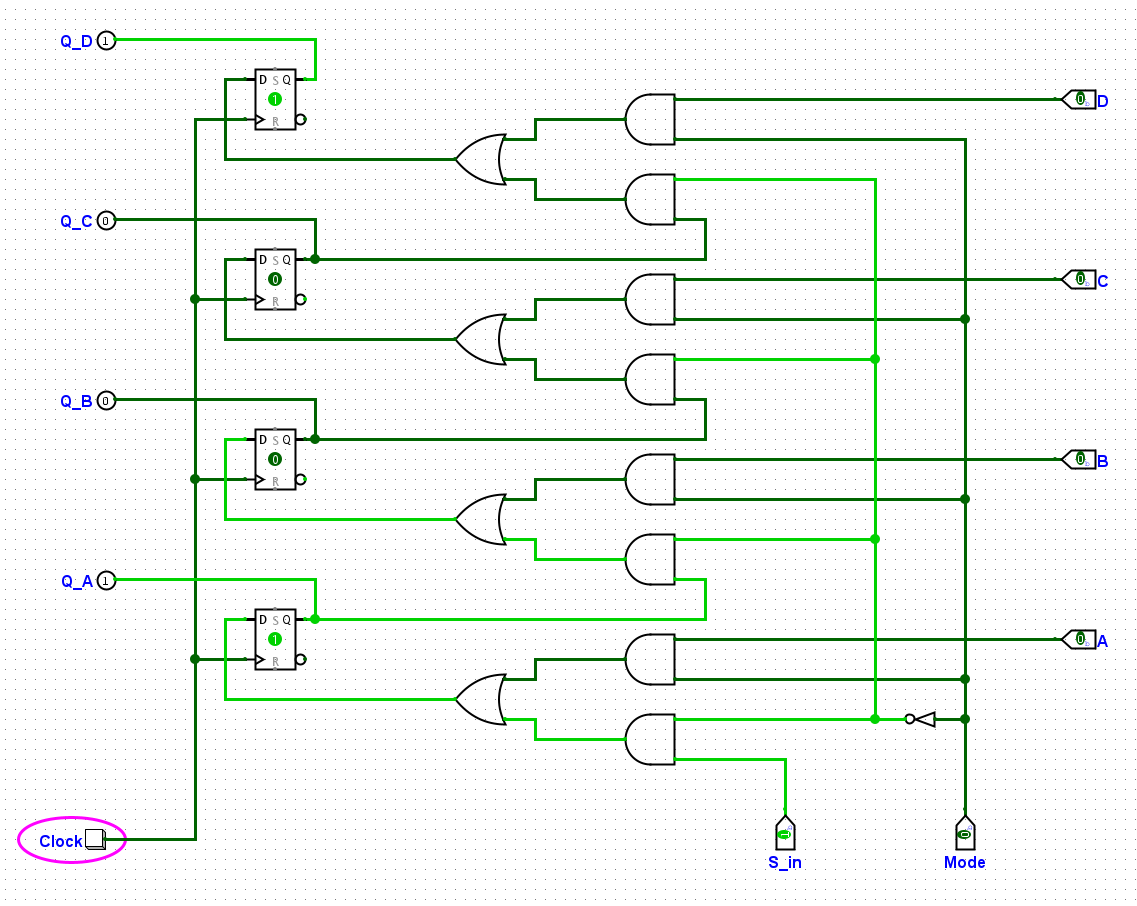
\includegraphics[width=\textwidth]{Screenshot 2026-08-09 160510.png}
		\caption{تیک چهارم و پنجم}
		\label{fig:rightshift-3-logisim}
	\end{subfigure}
	
	\caption{نمایش قدم به قدم وارد شدن مقدار $S_{in}$ به ازای هر تیک و شیفت به سمت راست}
	\label{fig:rightshift-example-logisim}
\end{figure}

\begin{figure}[htbp]
	\centering
	\begin{subfigure}[b]{0.48\textwidth}
		\centering
		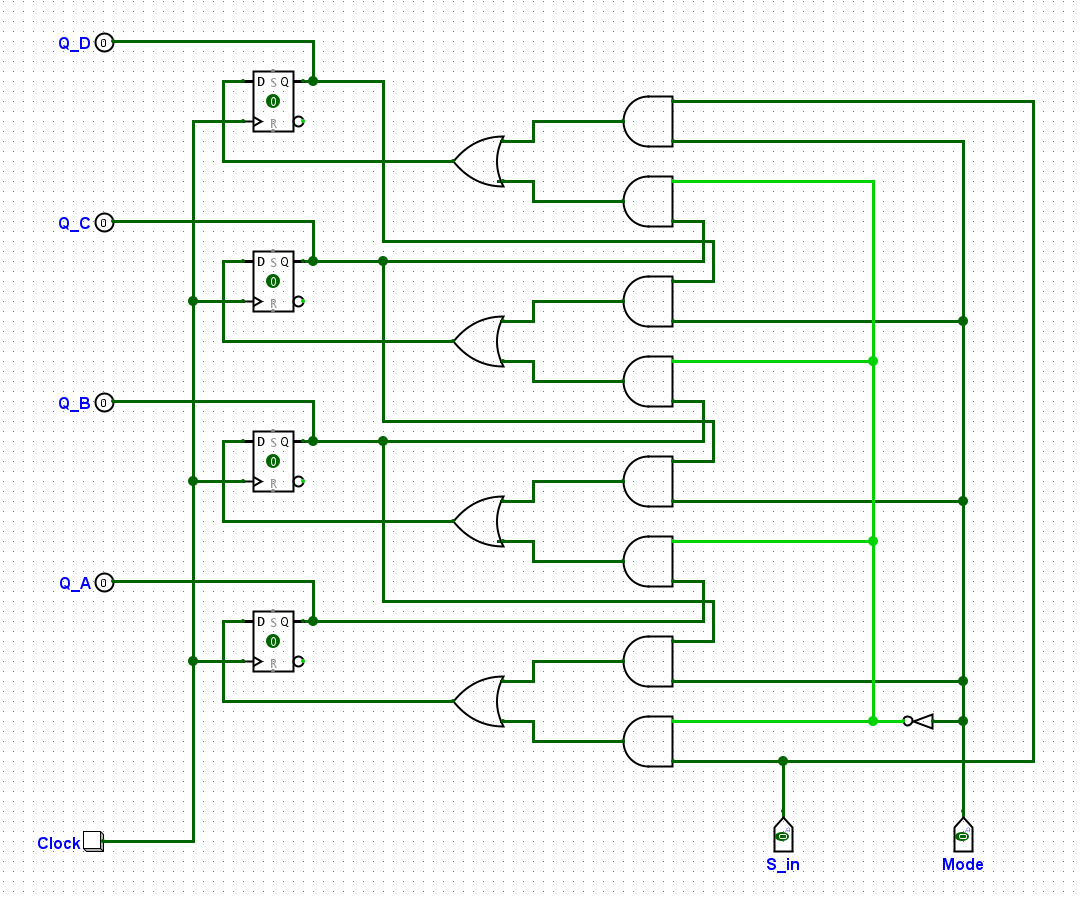
\includegraphics[width=\textwidth]{Screenshot 2026-08-09 160939.png}
		\caption{تیک اول -- شیفت چپ $Mode=1$}
		\label{fig:twoway-1-logisim}
	\end{subfigure}
	\hfill
	\begin{subfigure}[b]{0.48\textwidth}
		\centering
		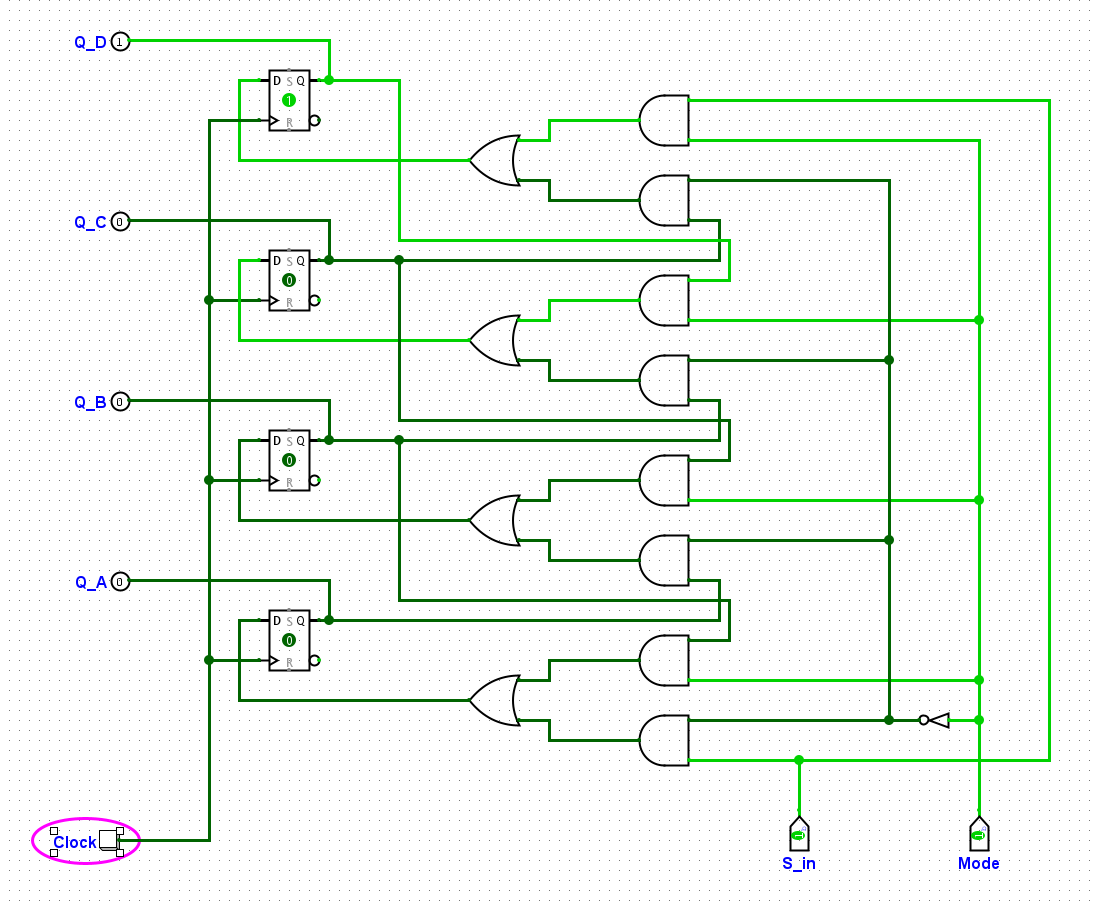
\includegraphics[width=\textwidth]{Screenshot 2026-08-09 161030.png}
		\caption{تیک دوم -- شیفت چپ $Mode=1$}
		\label{fig:twoway-2-logisim}
	\end{subfigure}
	
	\vspace{1em}
	
	\begin{subfigure}[b]{0.48\textwidth}
		\centering
		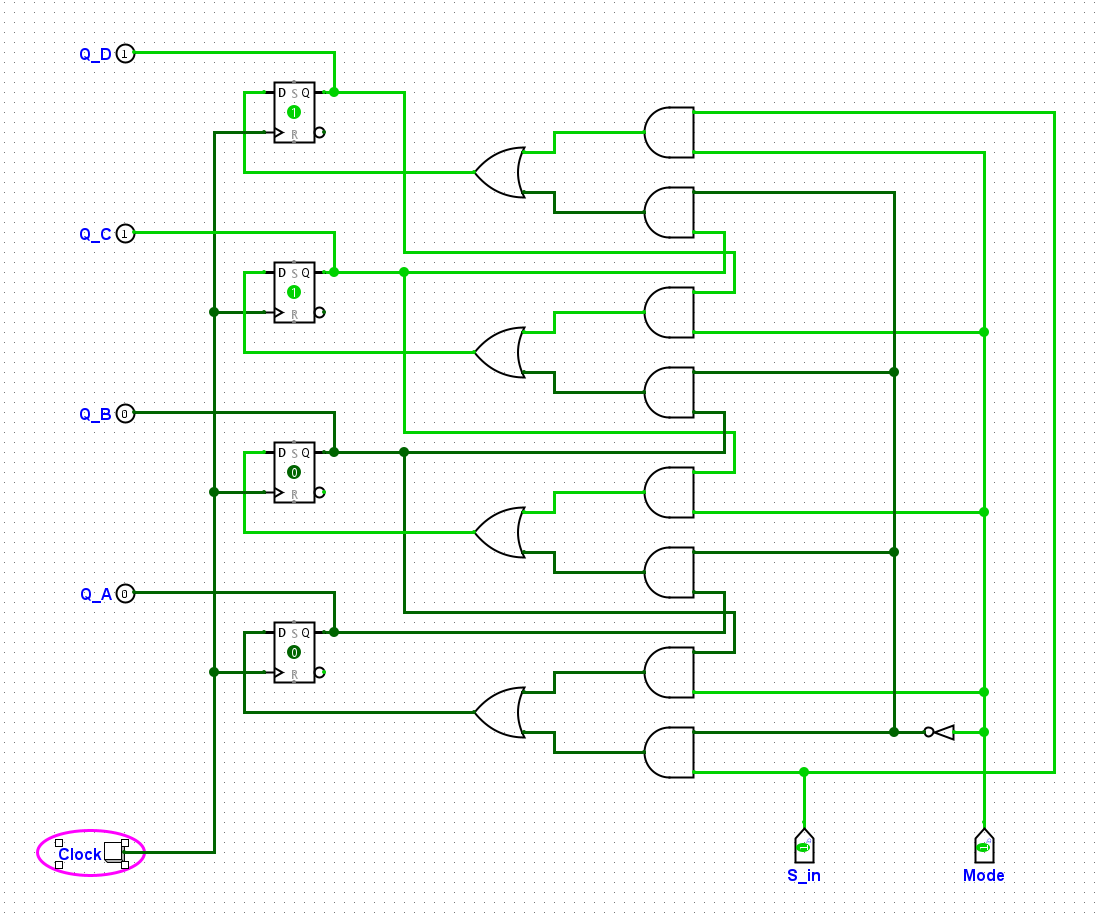
\includegraphics[width=\textwidth]{Screenshot 2026-08-09 161039.png}
		\caption{تیک سوم -- شیفت چپ $Mode=1$}
		\label{fig:twoway-3-logisim}
	\end{subfigure}
	\hfill
	\begin{subfigure}[b]{0.48\textwidth}
		\centering
		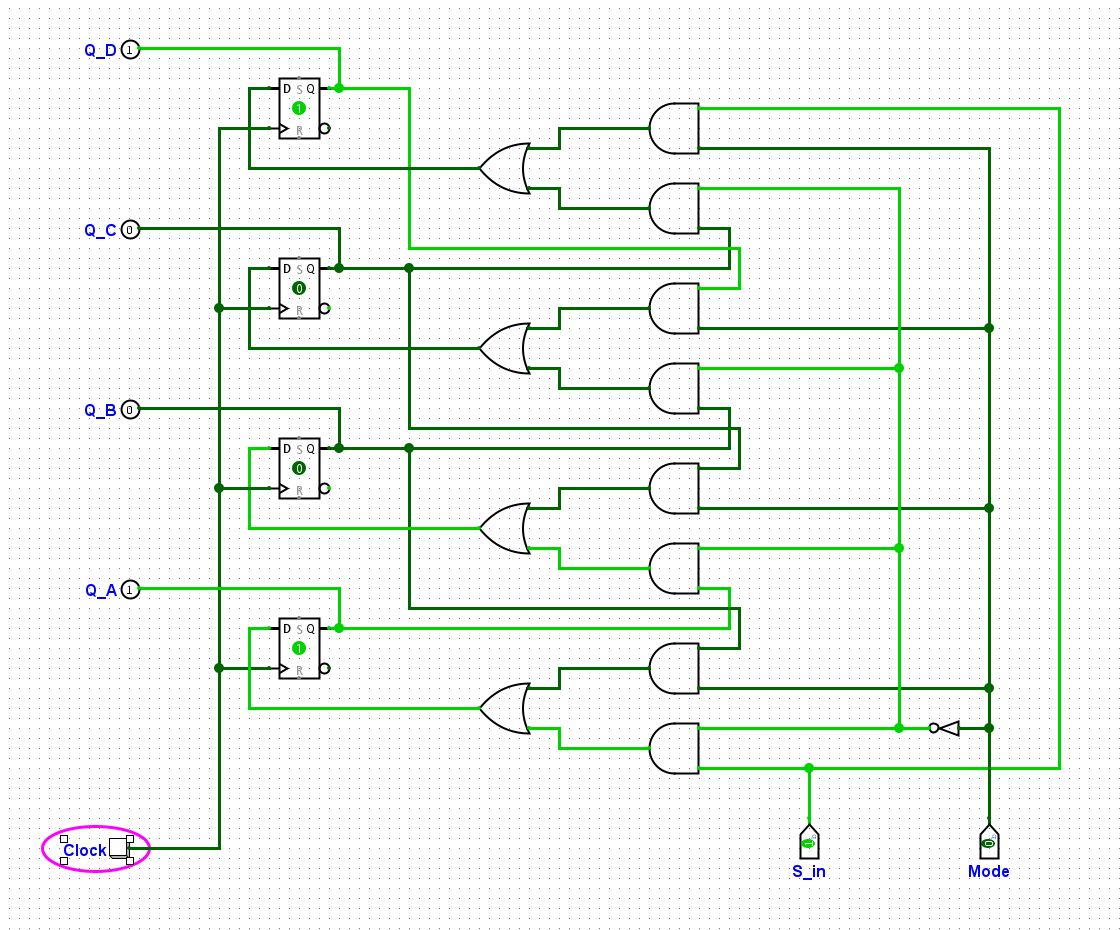
\includegraphics[width=\textwidth]{Screenshot 2026-08-09 161049.png}
		\caption{تیک چهارم -- شیفت راست $Mode=0$}
		\label{fig:twoway-4-logisim}
	\end{subfigure}
	
	\caption{نمایش شیفت دو طرفه}
	\label{fig:twoway-example-logisim}
\end{figure}

\clearpage

\section{استفاده از شیفت رجیستر آماده}

\subsection{طراحی در پروتئوس}

\subsubsection{تراشه 7495}

در این بخش باید برای ساخت شیفت رجیستر از تراشه آماده 7495 برای ساخت آن استفاده کنیم. خود تراشه یک شیفت رجیستر آماده ست و تقریبا تمام کار اصلی را انجام داده است. کافی است سیم کشی های لازم برای ورودی ها و کلاک ها و خروجی ها را انجام دهیم.

\begin{figure}[htbp]
	\centering
	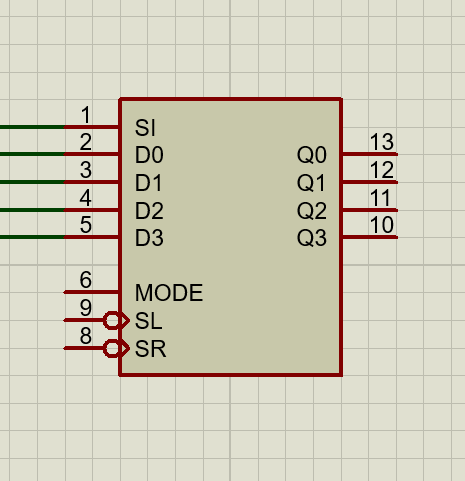
\includegraphics[width=0.8\textwidth]{Screenshot 2026-08-09 111550.png}
	\caption{تراشه 7495}
\end{figure}

\clearpage

پین 6 همان سوییچ $Mode$ است که به ازای 1 بارگذاری بیت های $D_0$ تا $D_3$ را انجام می دهد و به ازای 0 شیفت راست را انجام می دهد و مقدار سریال را از پین 1 ($SI$) می خواند. این تراشه به ازای هر مود کلاک مجزایی دارد. کلاک $SL$ که برای مود شیفت است و کلاک $SR$ که برای مود بارگذاری استفاده می شود. در نهایت این تراشه بعد از هر کلاک خروجی را در $Q_0$ تا $Q_3$ می ریزد. شایان ذکر است که کلاک مودی که نامعتبر است بی تاثیر است.

شایان ذکر است که $D_0$ در ورودی ها و $Q_0$ در خروجی ها MSB هستند.

بلوک‌دیاگرام این بخش در شکل~\ref{fig:block-7495} بسیار ساده‌تر از دو بخش قبل است، چرا که تمام منطق کنترل بارگذاری/شیفت درون خود تراشه پیاده‌سازی شده.

\begin{figure}[htbp]
    \centering
    \beginL
    \begin{tikzpicture}[node distance=0.6cm and 1.6cm]
        \node[block, minimum height=3.2cm, minimum width=3.2cm] (ic) {\RL{تراشه} 7495\\\RL{شیفت‌رجیستر ۴ بیتی}};
        \node[io, left=of ic, yshift=1.1cm] (si) {$S_I$};
        \node[io, left=of ic, yshift=0.35cm] (d) {$D_0..D_3$};
        \node[io, left=of ic, yshift=-0.4cm] (mode) {$MODE$};
        \node[io, left=of ic, yshift=-1.15cm] (clk) {$SL,\ SR$};
        \node[io, right=of ic] (out) {$Q_0..Q_3$};

        \draw[sig] (si) -- (ic);
        \draw[sig] (d) -- (ic);
        \draw[sig] (mode) -- (ic);
        \draw[sig] (clk) -- (ic);
        \draw[sig] (ic) -- (out);
    \end{tikzpicture}
    \endL
    \caption{بلوک‌دیاگرام شیفت‌رجیستر مبتنی بر تراشهٔ 7495}
    \label{fig:block-7495}
\end{figure}

\clearpage

بعد از سیم کشی های لازم نتیجه به این صورت است:

\begin{figure}[htbp]
	\centering
	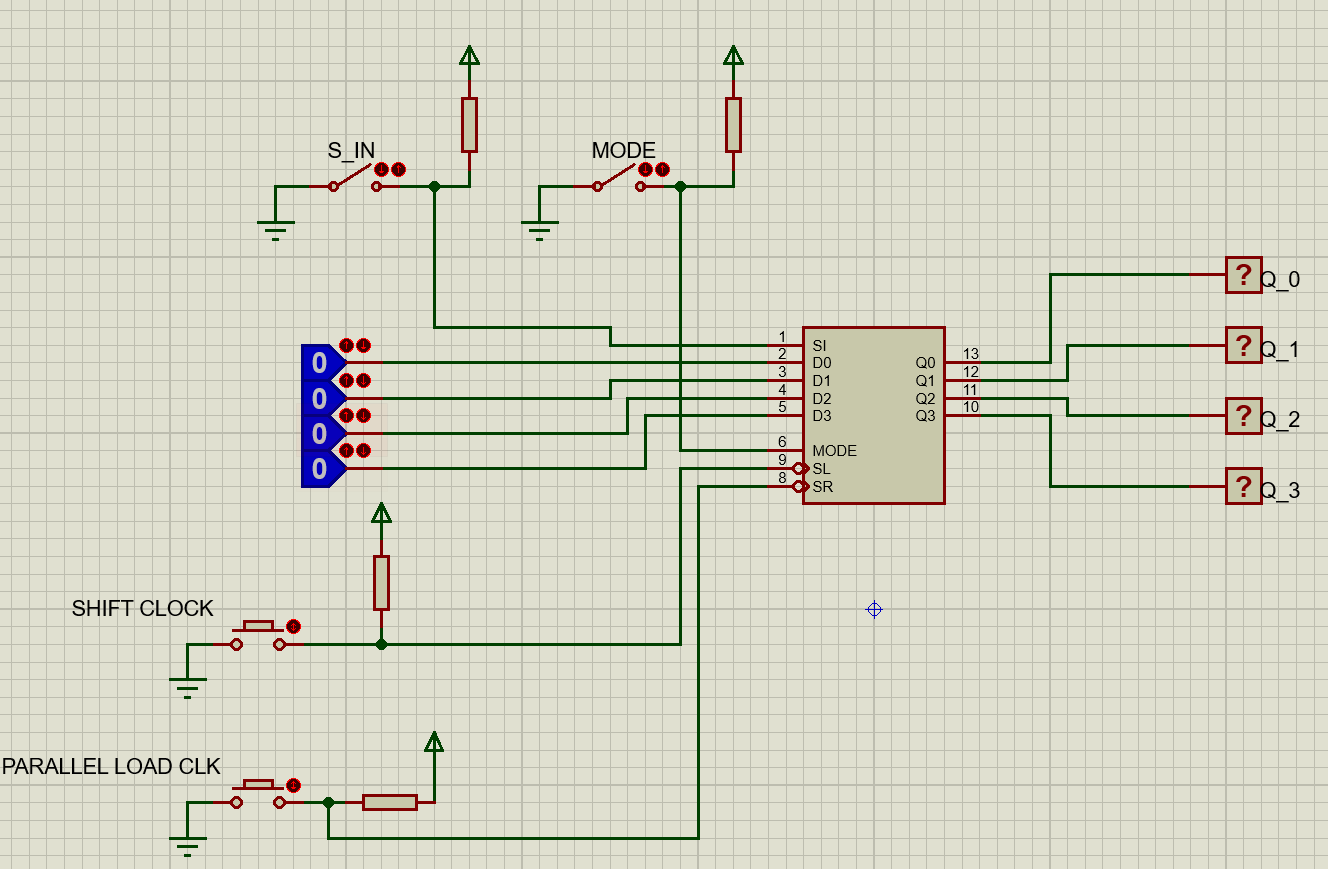
\includegraphics[width=0.98\textwidth]{Screenshot 2026-08-09 121504.png}
	\caption{پیاده سازی شیفت رجیستر با تراشه 7459}
\end{figure}

\begin{figure}[htbp]
	\centering
	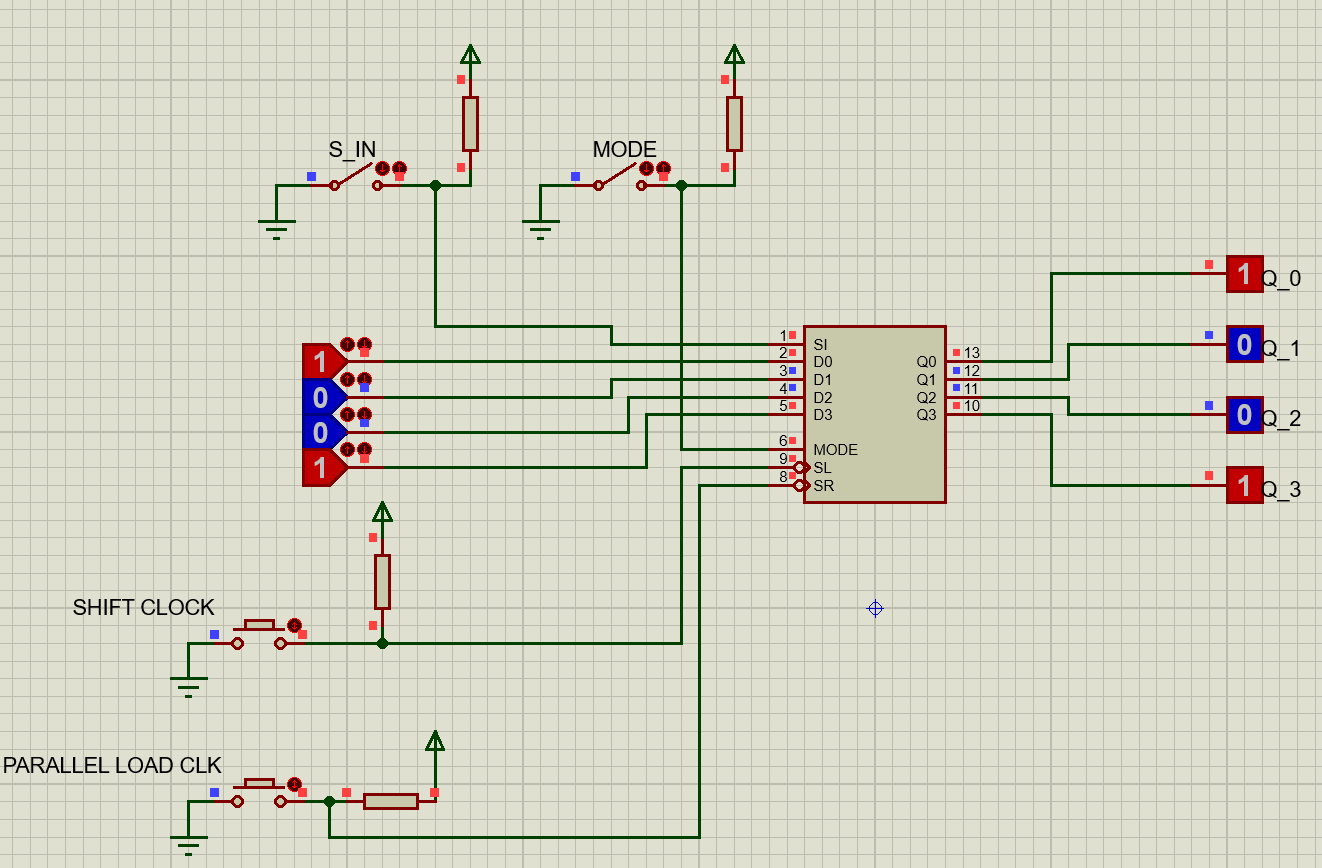
\includegraphics[width=0.98\textwidth]{Screenshot 2026-08-09 121517.png}
	\caption{بارگذاری عدد 1001 در شیفت رجیستر}
\end{figure}


\begin{figure}[htbp]
	\centering
	\begin{subfigure}[b]{0.48\textwidth}
		\centering
		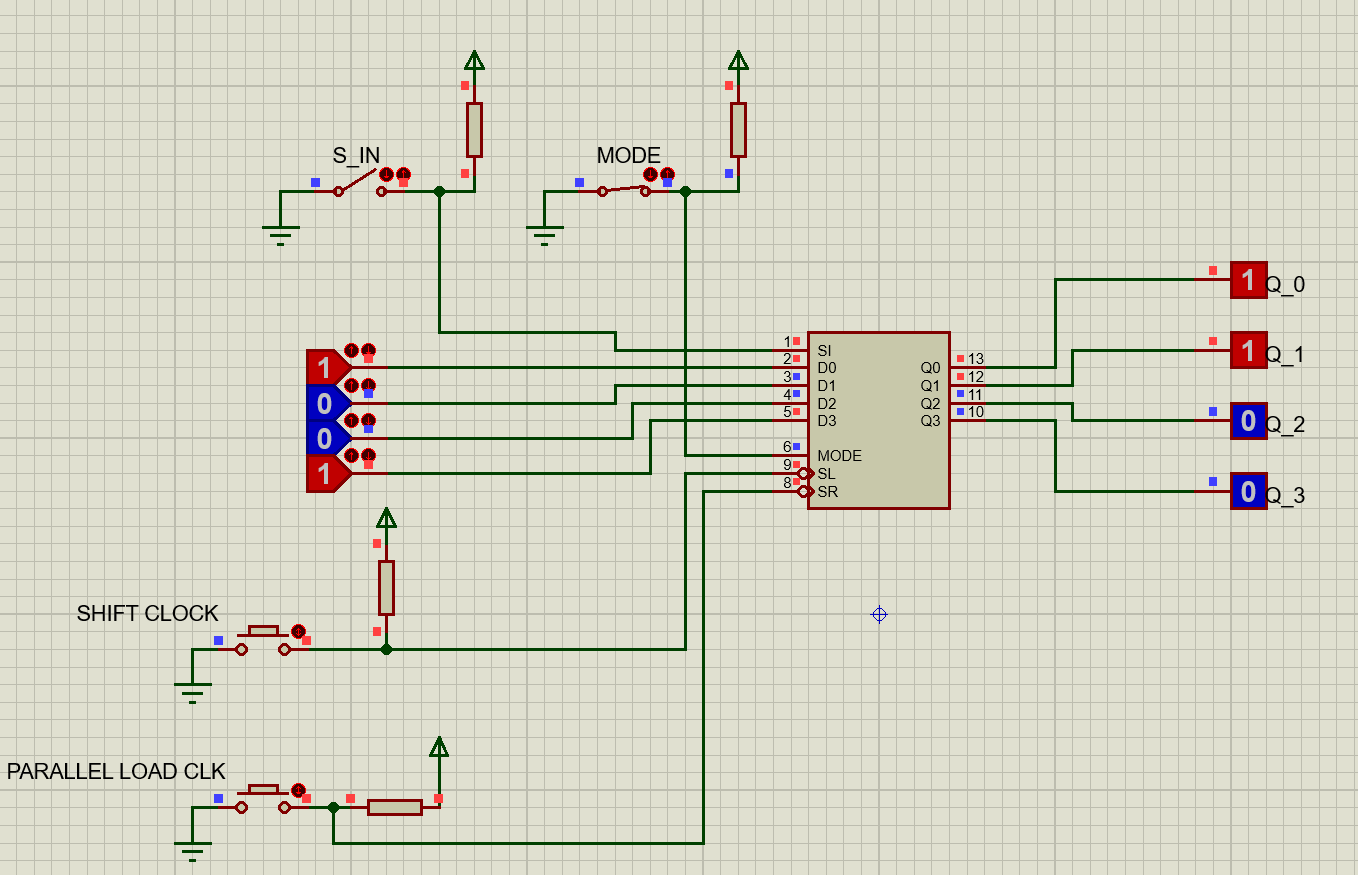
\includegraphics[width=\textwidth]{Screenshot 2026-08-09 121531.png}
		\caption{تیک اول}
		\label{fig:rightshift-1-7459-proteus}
	\end{subfigure}
	\hfill
	\begin{subfigure}[b]{0.48\textwidth}
		\centering
		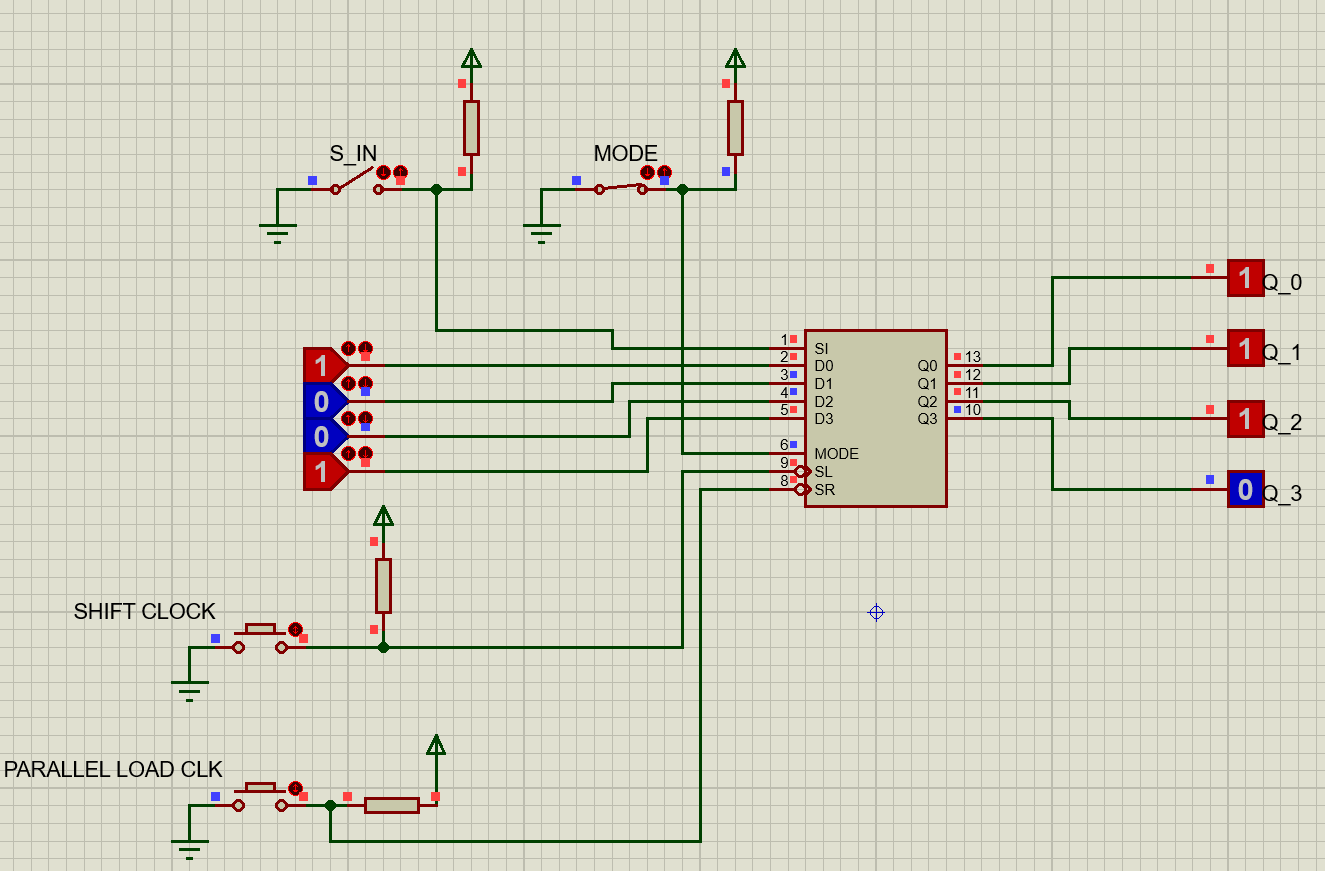
\includegraphics[width=\textwidth]{Screenshot 2026-08-09 121544.png}
		\caption{تیک دوم}
		\label{fig:rightshift-2-7459-proteus}
	\end{subfigure}
	
	\vspace{1em}
	
	\begin{subfigure}[b]{0.48\textwidth}
		\centering
		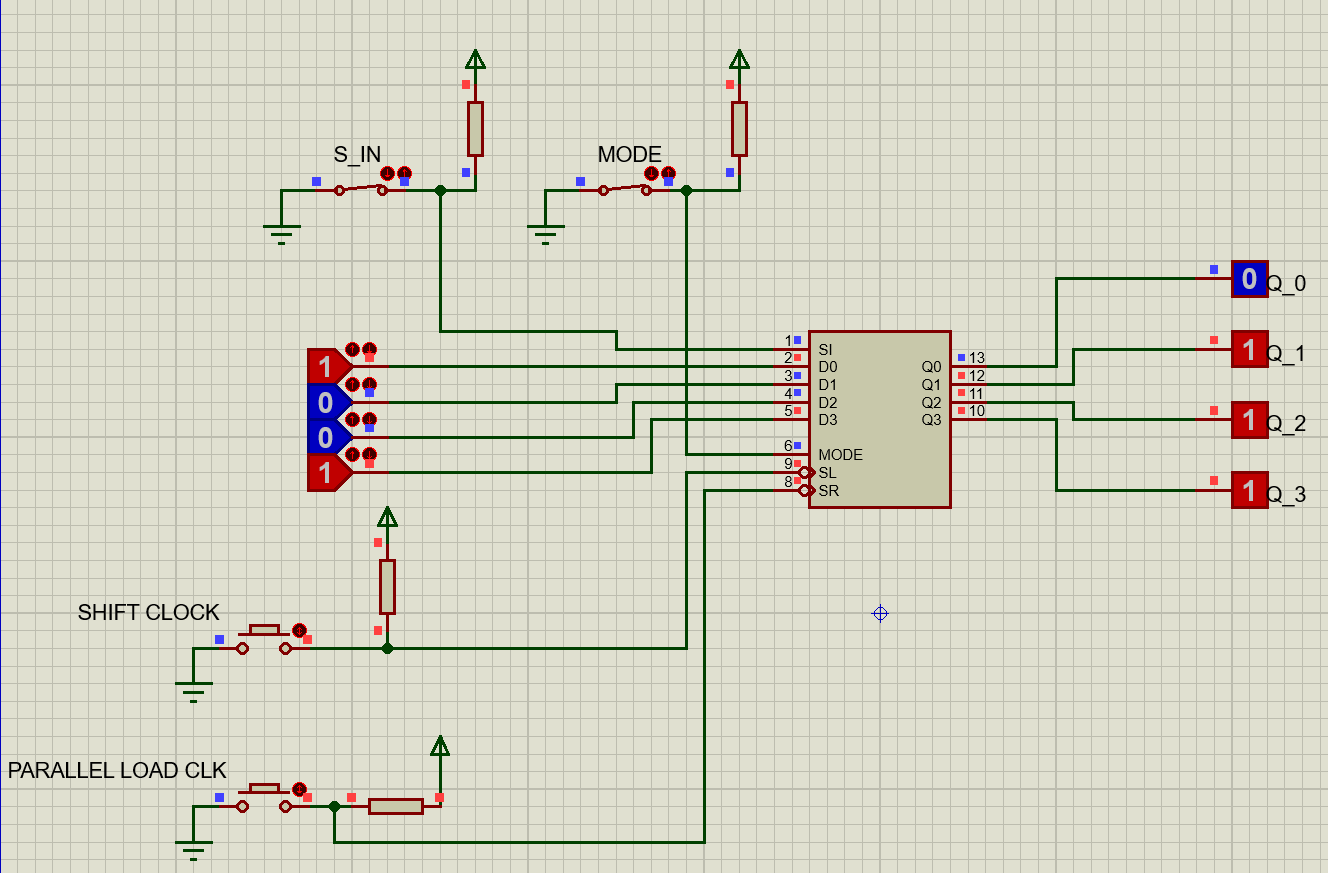
\includegraphics[width=\textwidth]{Screenshot 2026-08-09 121554.png}
		\caption{تیک سوم}
		\label{fig:rightshift-3-7459-proteus}
	\end{subfigure}
	
	\caption{نمایش قدم به قدم وارد شدن مقدار $S_{in}$ به ازای هر تیک و شیفت به سمت راست}
	\label{fig:rightshift-example-7459-proteus}
\end{figure}

\clearpage

\subsubsection{تشخیص رشته}
در بخش بعدی از ما خواسته شده که رشته های 1101، 1110، 0010، 0001 را در خروجی شیفت رجیستر تشخیص دهیم و مقدار 1 را به ازای آنها نمایش دهیم.

برای این کار اول جدول درستی مربوط به این رشته ها و خروجی را رسم می کنیم:

\begin{figure}[htbp]
	\centering
	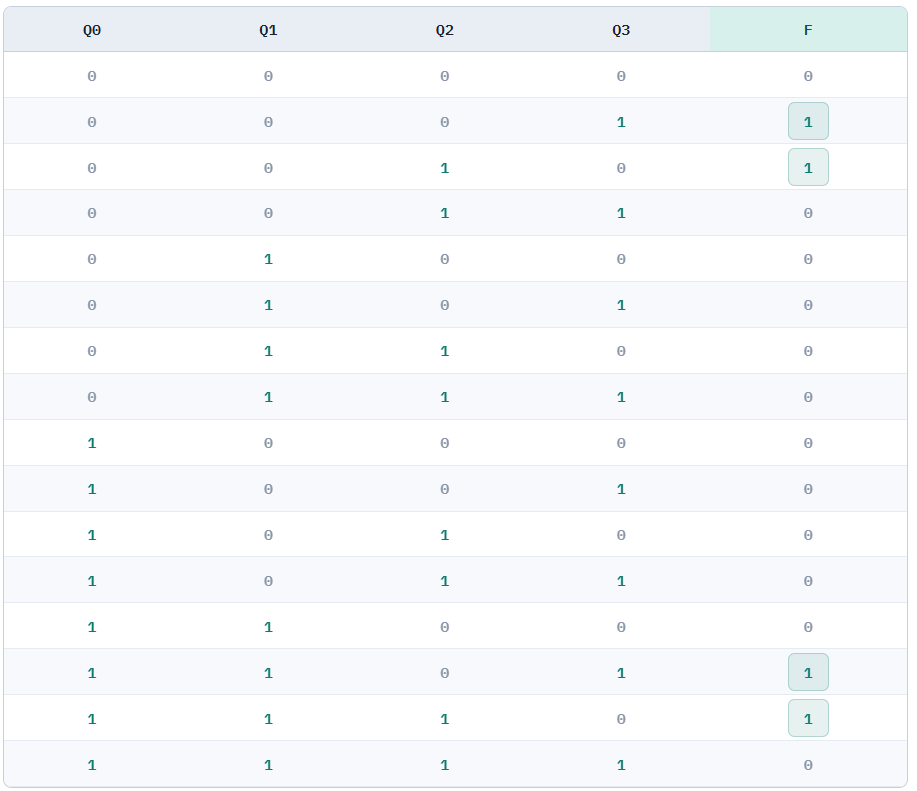
\includegraphics[width=0.98\textwidth]{Screenshot 2026-08-09 150654.png}
	\caption{جدول درستی رشته های مدنظر}
\end{figure}

پس از محاسبه SOP مربوط به F، می رسیم به:
\[ F = Q_0'Q_1'Q_2'Q_3 + Q_0'Q_1'Q_2Q_3' + Q_0Q_1Q_2'Q_3 + Q_0Q_1Q_2Q_3' \]

بلوک‌دیاگرام کلی این بخش در شکل~\ref{fig:block-detector} نشان داده شده است.

\begin{figure}[htbp]
    \centering
    \beginL
    \begin{tikzpicture}[node distance=0.6cm and 1.6cm]
        \node[io] (in) {$D_0..D_3$\\\RL{کلاک‌ها}};
        \node[block, right=of in, minimum width=3cm] (sr) {\RL{شیفت‌رجیستر}\\(7495)};
        \node[block, right=of sr, minimum width=3.2cm] (det) {\RL{واحد ترکیبی}\\\RL{تشخیص رشته}\\(SOP از $Q_0..Q_3$)};
        \node[io, right=of det] (f) {$F$};

        \draw[sig] (in) -- (sr);
        \draw[sig] (sr) -- node[above]{$Q_0..Q_3$} (det);
        \draw[sig] (det) -- (f);
    \end{tikzpicture}
    \endL
    \caption{بلوک‌دیاگرام مدار تشخیص رشته}
    \label{fig:block-detector}
\end{figure}

سپس با توجه به آن گیت های مورد نیاز را قرار می دهیم و متصل می کنیم:

\begin{figure}[htbp]
	\centering
	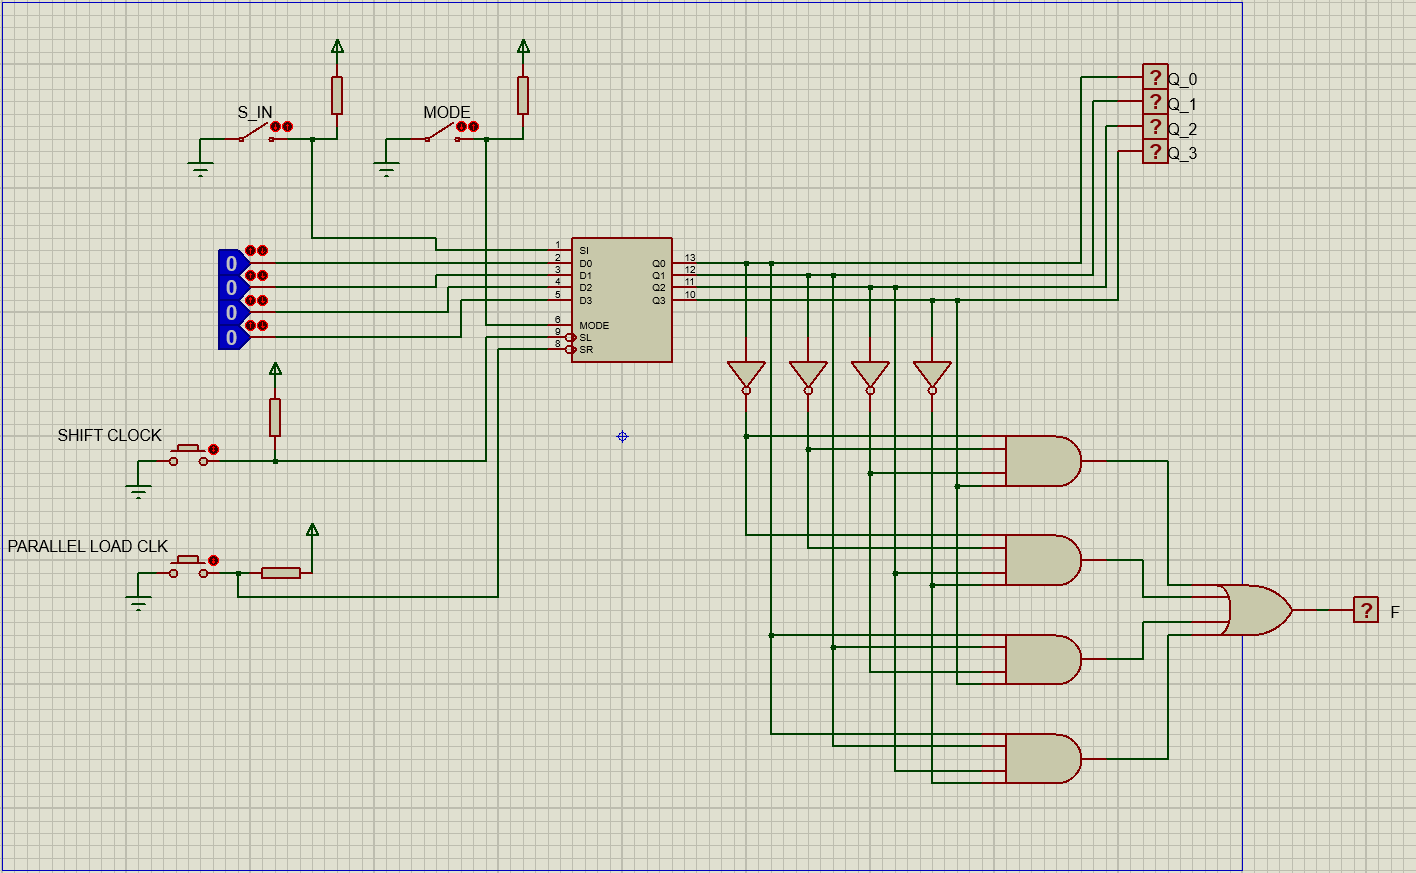
\includegraphics[width=0.8\textwidth, height=0.3\textheight]{Screenshot 2026-08-09 151917.png}
	\caption{مدار تشخیص رشته}
\end{figure}

\begin{figure}[htbp]
	\centering
	\begin{subfigure}[b]{0.48\textwidth}
		\centering
		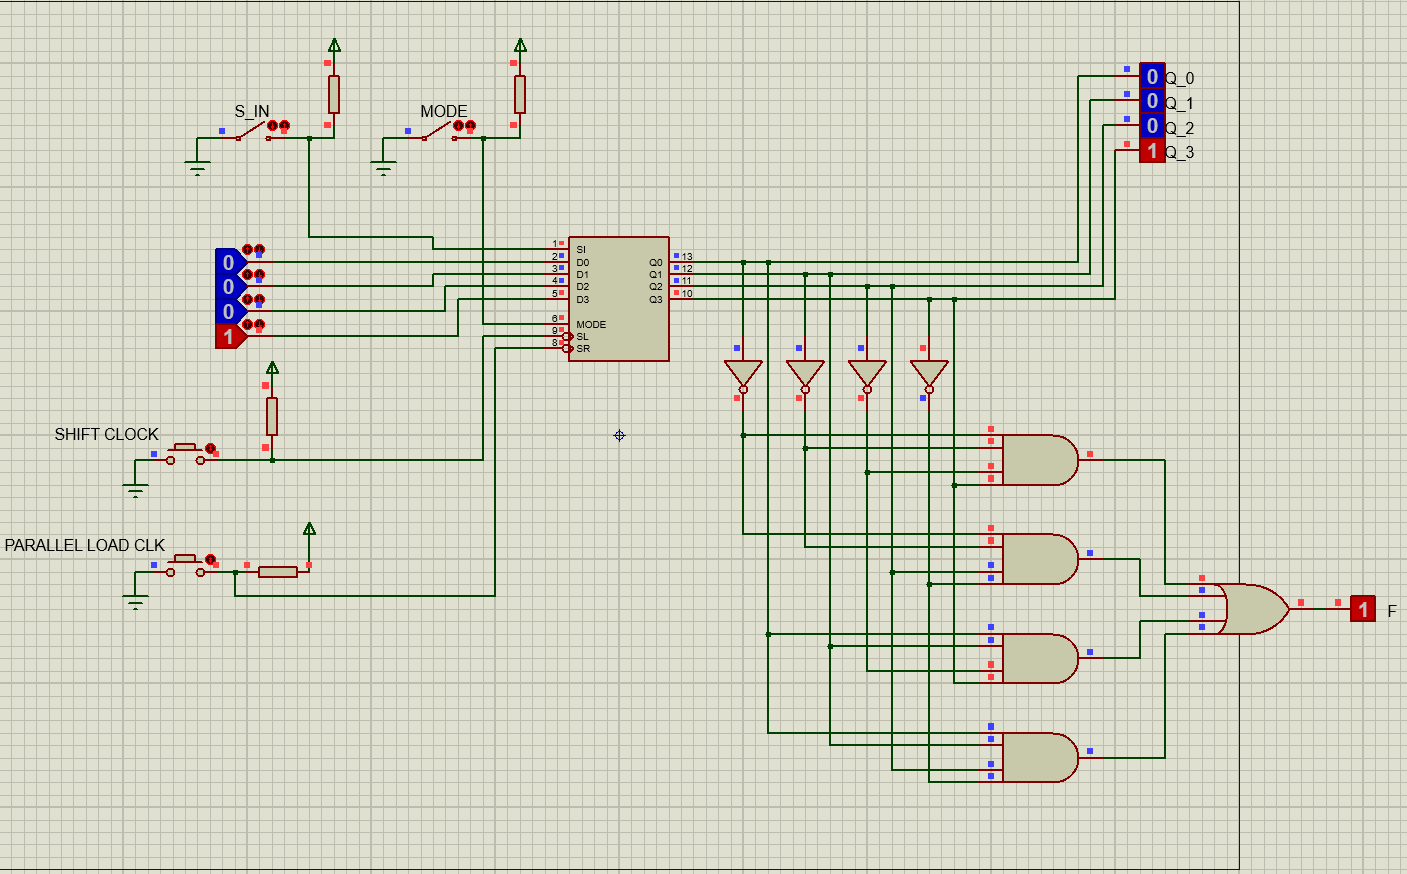
\includegraphics[width=\textwidth]{Screenshot 2026-08-09 152022.png}
		\caption{رشته 1000}
	\end{subfigure}
	\hfill
	\begin{subfigure}[b]{0.48\textwidth}
		\centering
		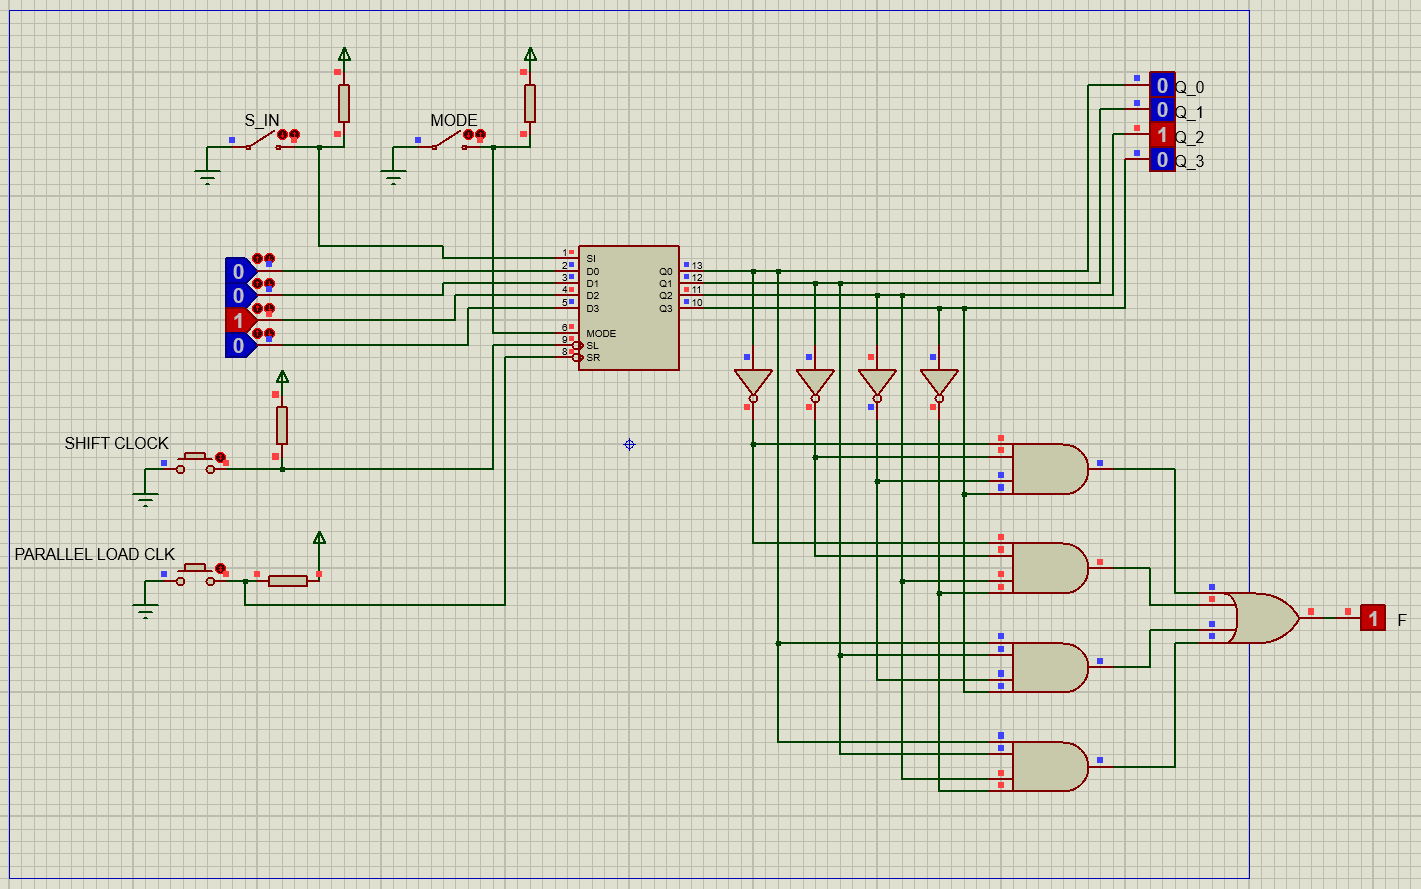
\includegraphics[width=\textwidth]{Screenshot 2026-08-09 152043.png}
		\caption{رشته 0100}
	\end{subfigure}
	
	\vspace{1em}
	
	\begin{subfigure}[b]{0.48\textwidth}
		\centering
		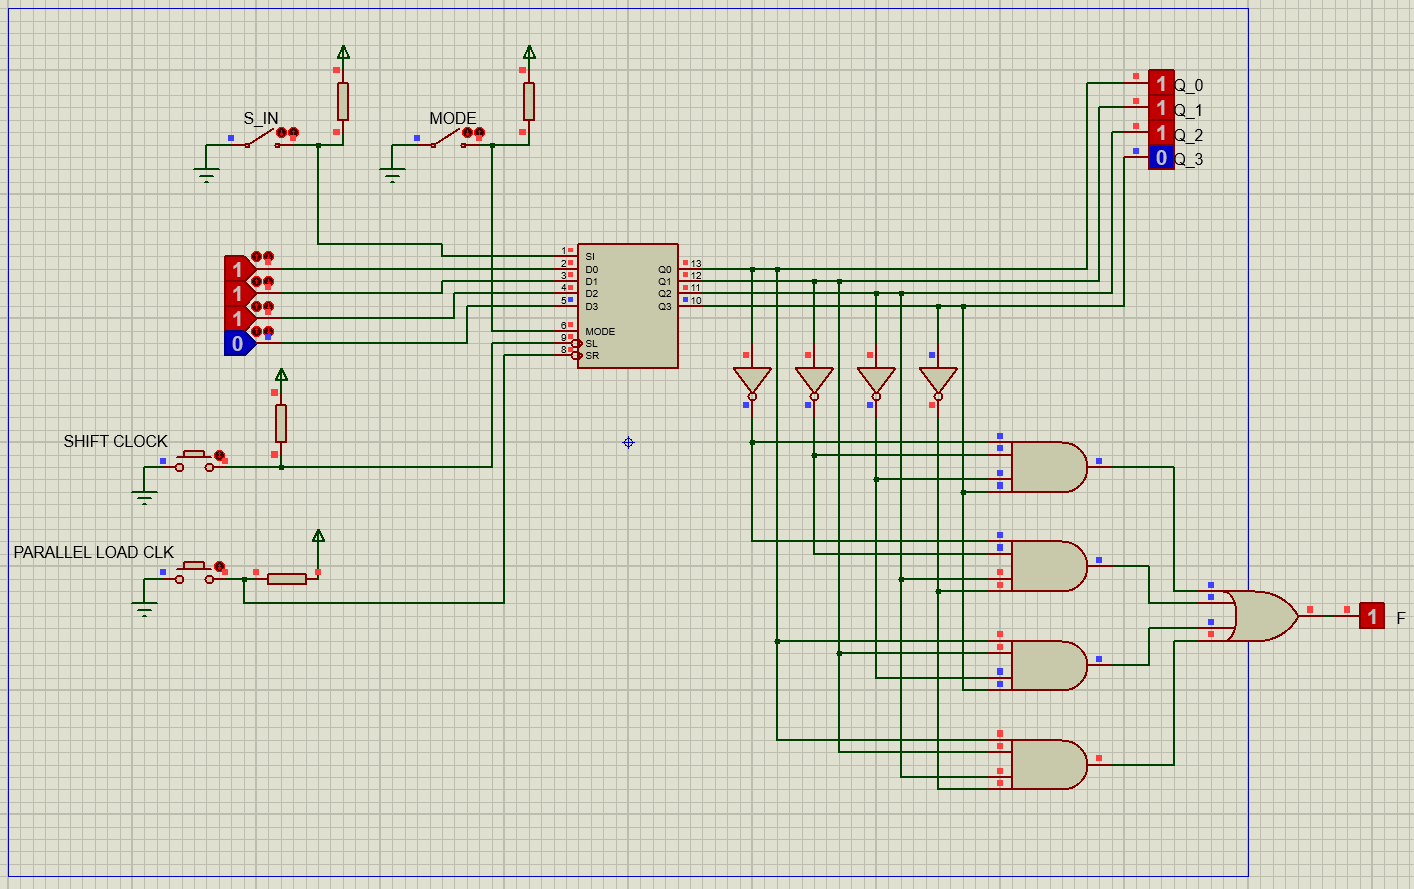
\includegraphics[width=\textwidth]{Screenshot 2026-08-09 152059.png}
		\caption{رشته 0111}
	\end{subfigure}
	\hfill
	\begin{subfigure}[b]{0.48\textwidth}
		\centering
		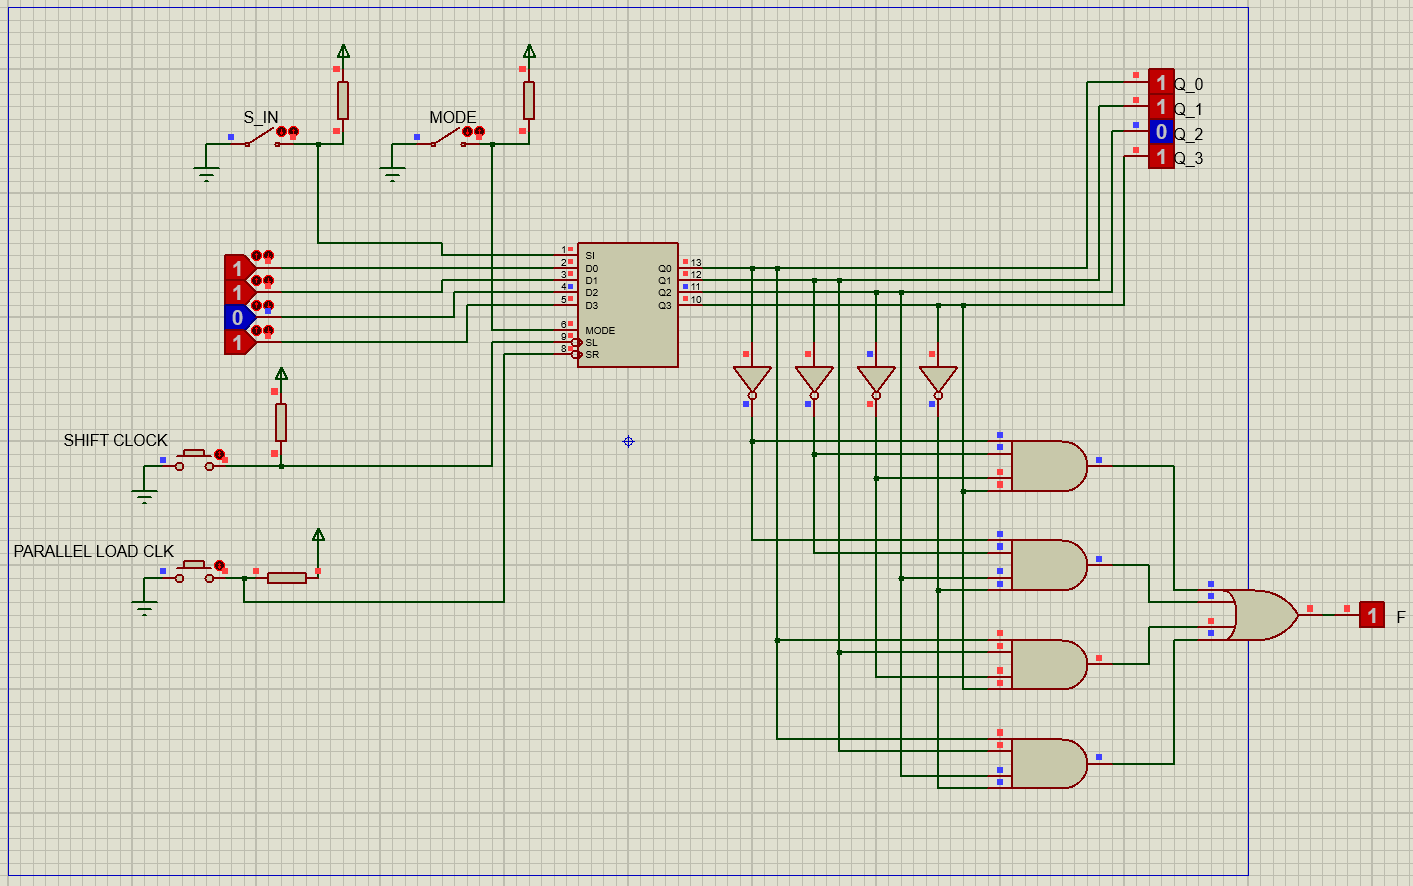
\includegraphics[width=\textwidth]{Screenshot 2026-08-09 152111.png}
		\caption{رشته 1011}
	\end{subfigure}
	
	\caption{نمایش تشخیص رشته های مد نظر}
\end{figure}

\begin{figure}[htbp]
		\centering
		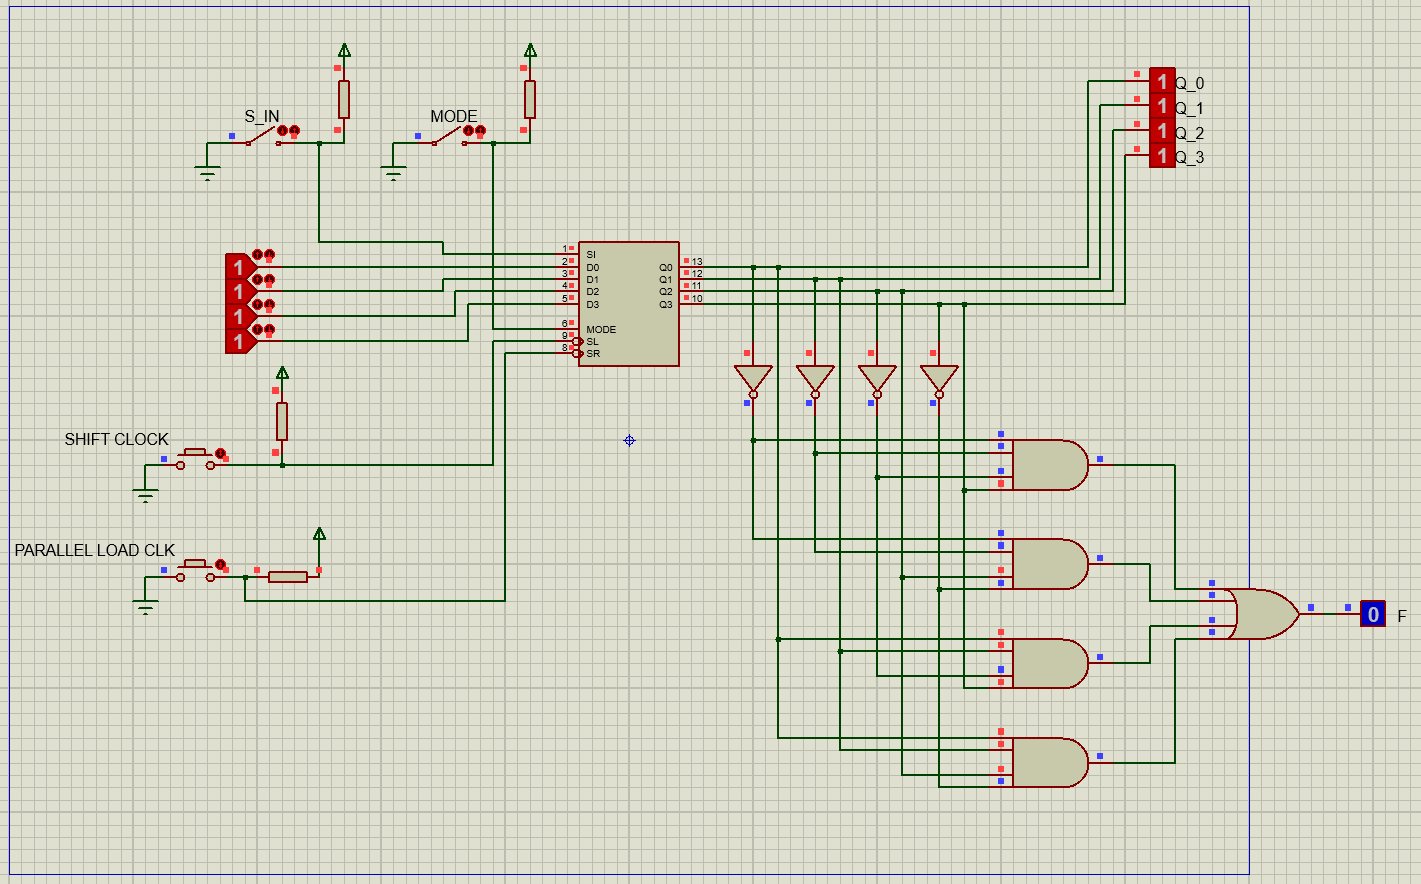
\includegraphics[width=\textwidth]{Screenshot 2026-08-09 152119.png}
	\caption{نمایش خروجی 0 به ازای رشته نامعتبر}
\end{figure}

\clearpage

\subsection{طراحی در لاجیسیم}

در لاجیسیم تراشه 7495 موجود نیست. در نتیجه برای نمایش کارکرد آن لازم است نمونه ای معادل پیاده سازی کنیم. از آنجا که کارکرد آن تقریبا با شیفت رجیستری که با استفاده از 4 فلیپ فلاپ پیاده سازی کرده بودیم یکسان است و تنها در وجود دو کلاک متفاوت به ازای هر mode تفاوت دارد، لازم است این دو کلاک را به گونه ای اضافه کنیم که تنها به ازای mode مربوط به خود عمل کنند.

برای تشخیص رشته های 1101، 1110، 0010، 0001 نیز مانند قبل عمل می کنیم.

مانند قبل $A$ ، MSB است.

\begin{figure}[htbp]
	\centering
	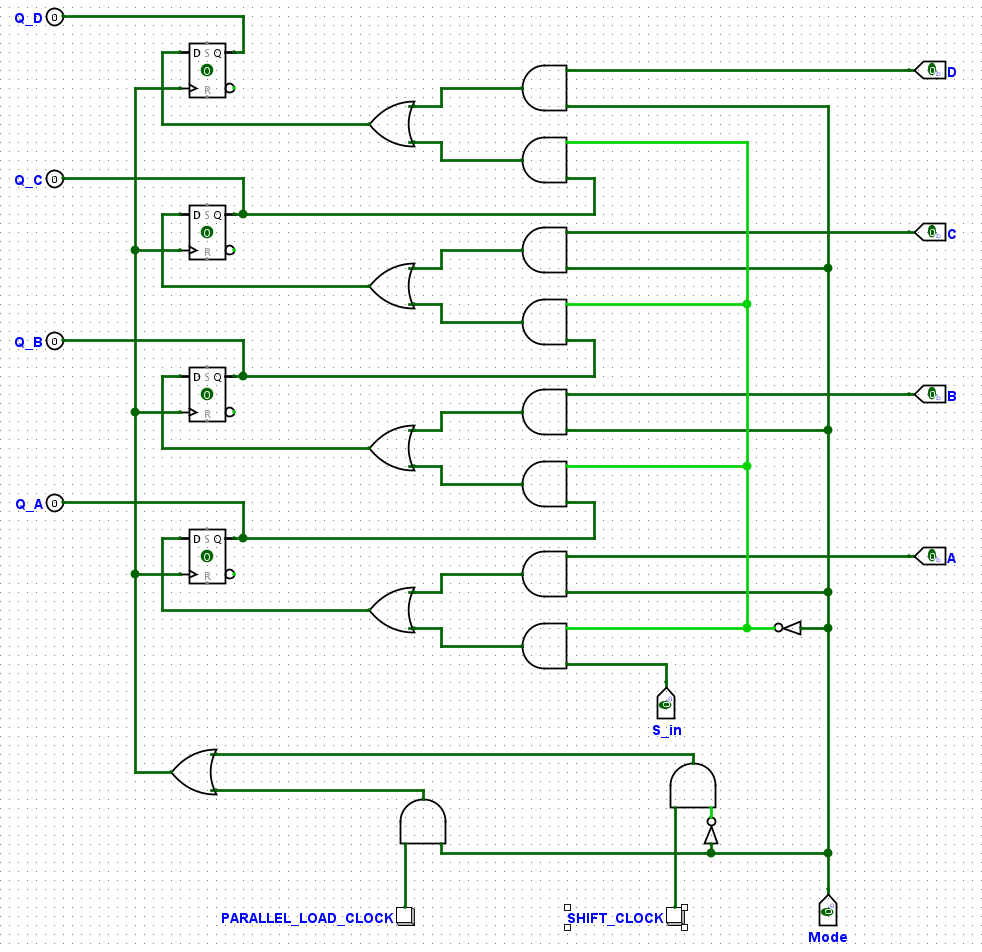
\includegraphics[width=\textwidth]{Screenshot 2026-08-09 165324.png}
	\caption{پیاده سازی شیفت رجیستر با دو کلاک در لاجیسیم}
\end{figure}

\begin{figure}[htbp]
	\centering
	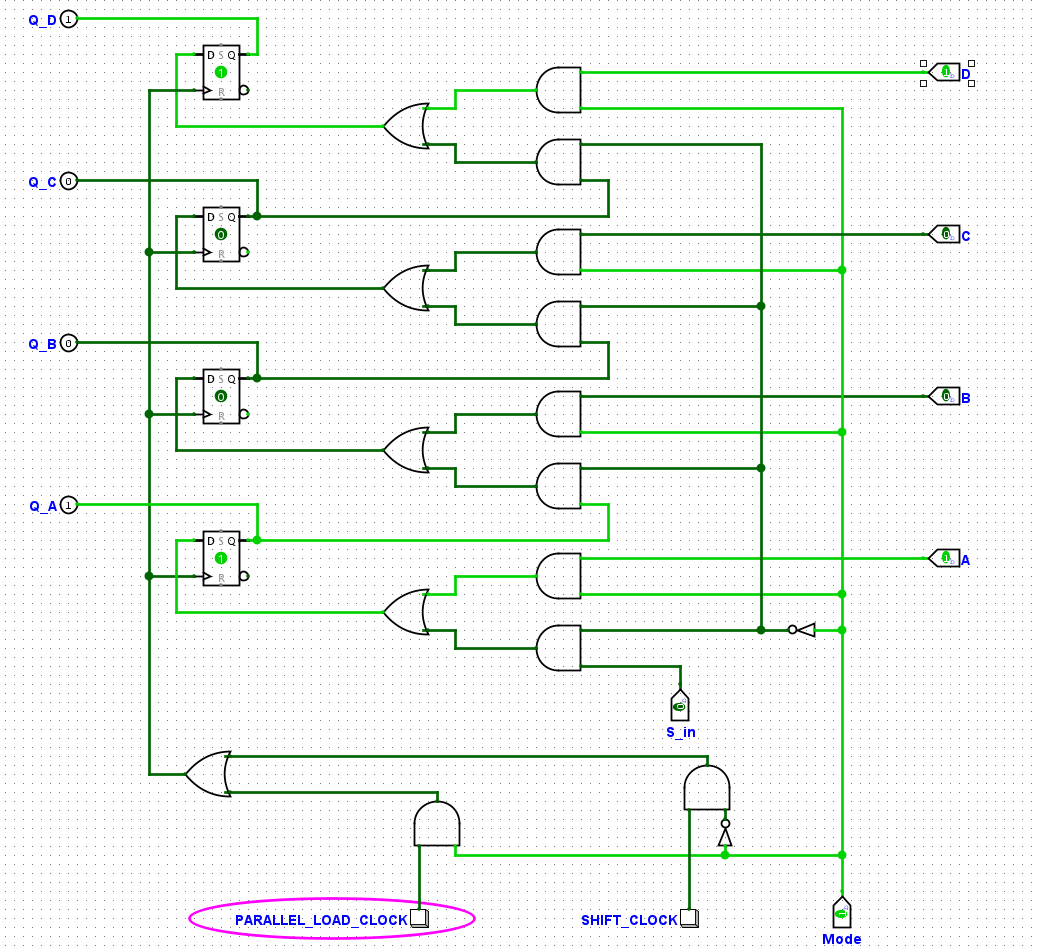
\includegraphics[width=\textwidth]{Screenshot 2026-08-09 165409.png}
	\caption{بارگذاری رشته 1001 در رجیستر}
\end{figure}

\begin{figure}[htbp]
	\centering
	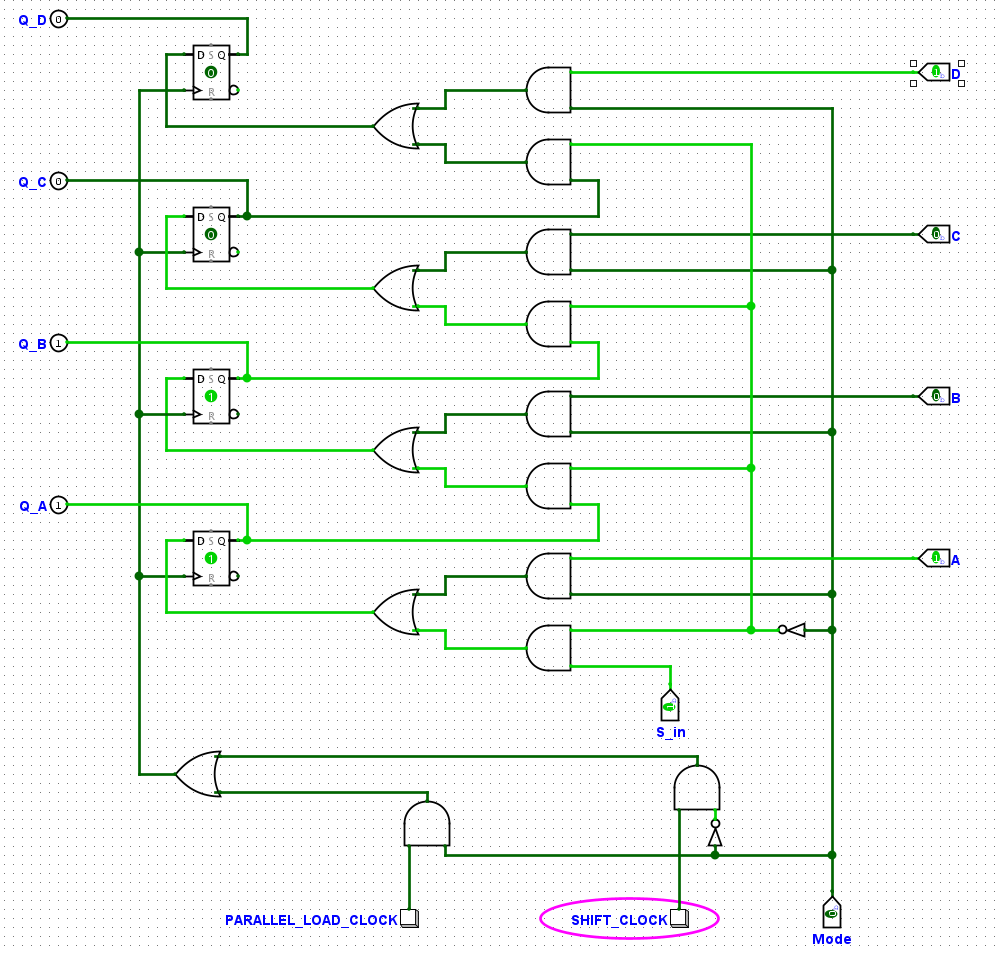
\includegraphics[width=\textwidth]{Screenshot 2026-08-09 165504.png}
	\caption{شیفت به بالا به ازای یک تیک کلاک}
\end{figure}

\begin{figure}[htbp]
	\centering
	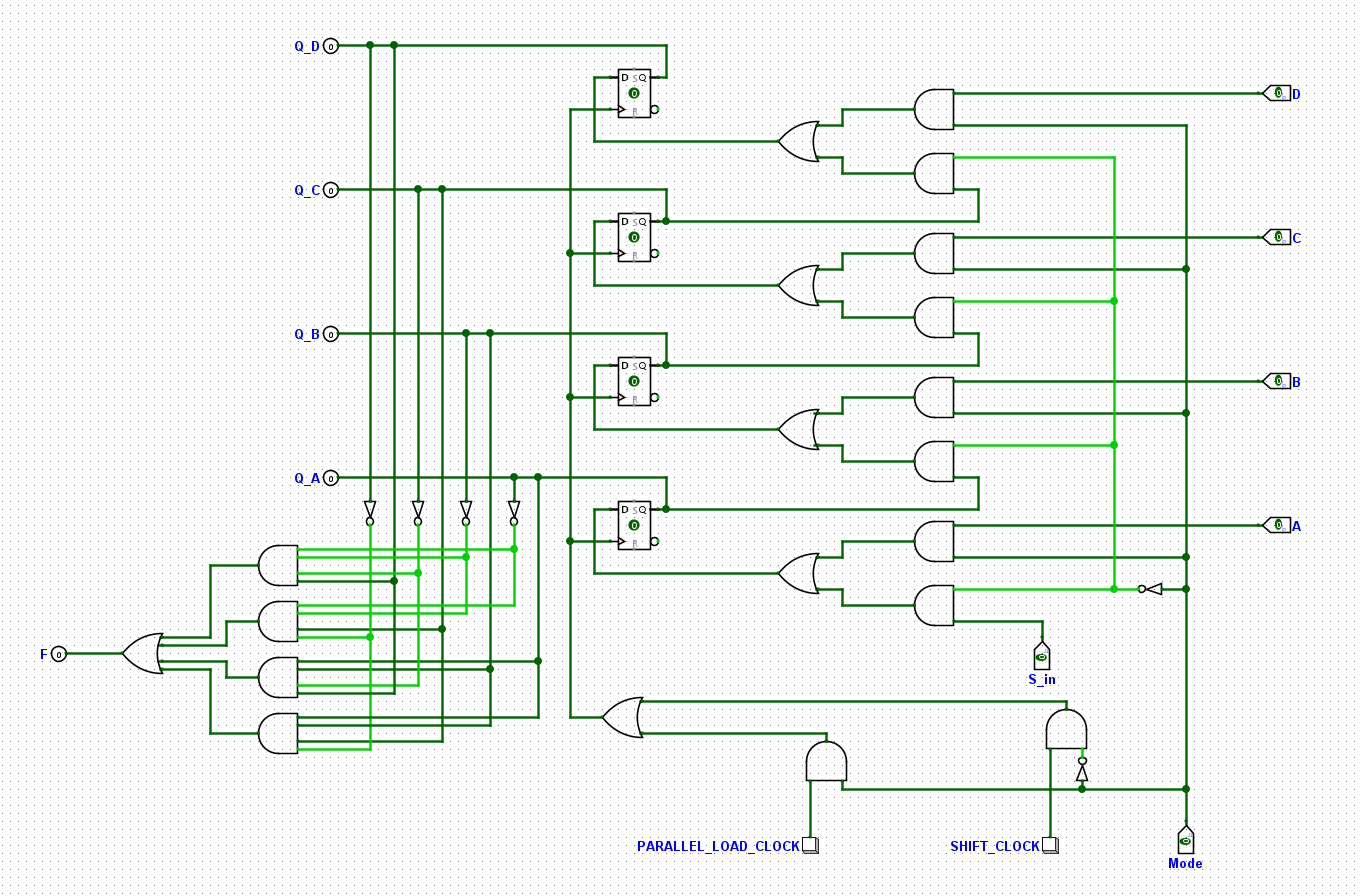
\includegraphics[width=\textwidth]{Screenshot 2026-08-09 171129.png}
	\caption{تشخیص رشته های 1101، 1110، 0010، 0001 در لاجیسیم}
\end{figure}

\begin{figure}[htbp]
	\centering
	\begin{subfigure}[b]{0.48\textwidth}
		\centering
		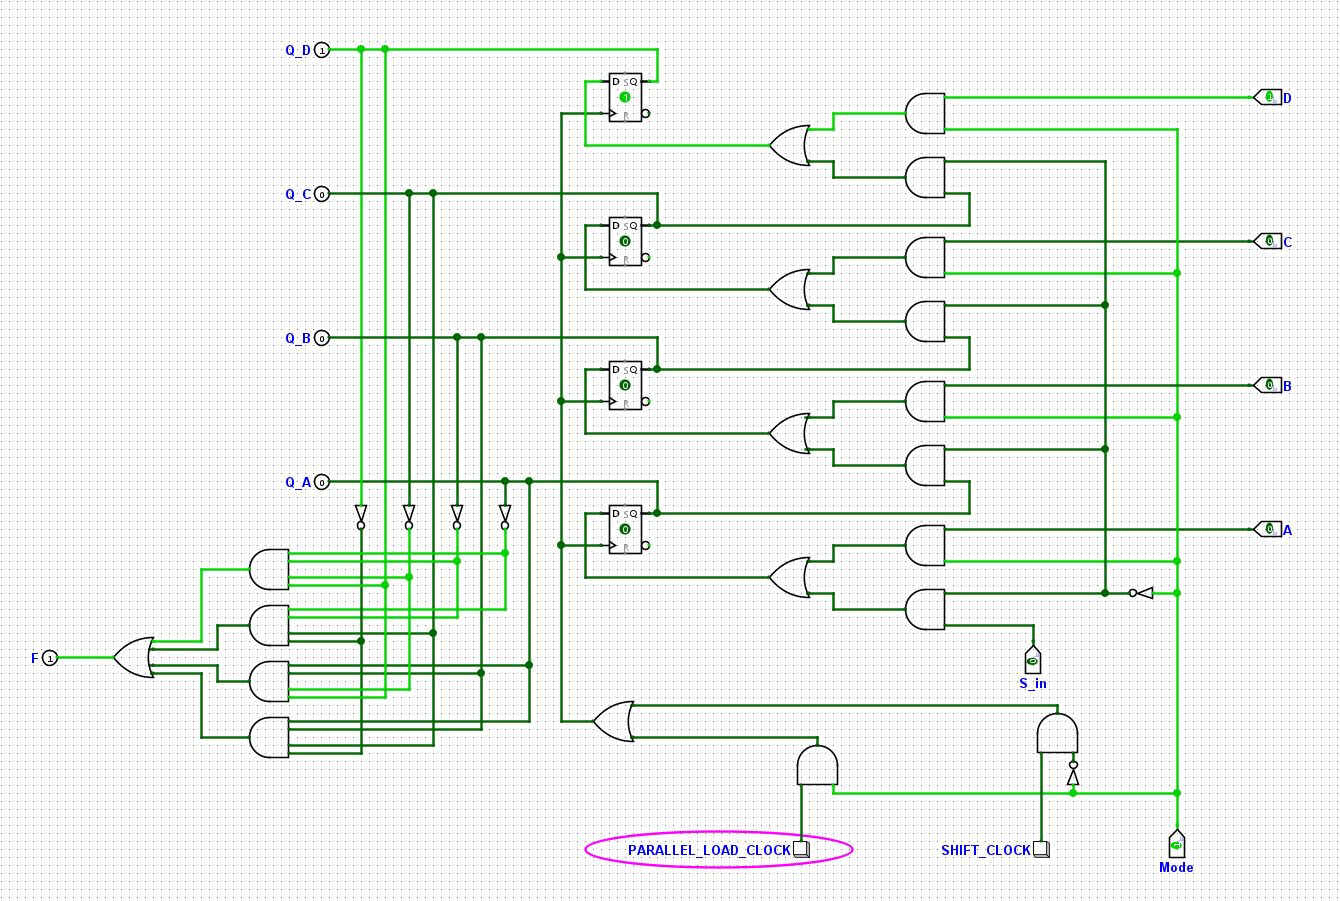
\includegraphics[width=\textwidth]{Screenshot 2026-08-09 171157.png}
		\caption{رشته 1000}
	\end{subfigure}
	\hfill
	\begin{subfigure}[b]{0.48\textwidth}
		\centering
		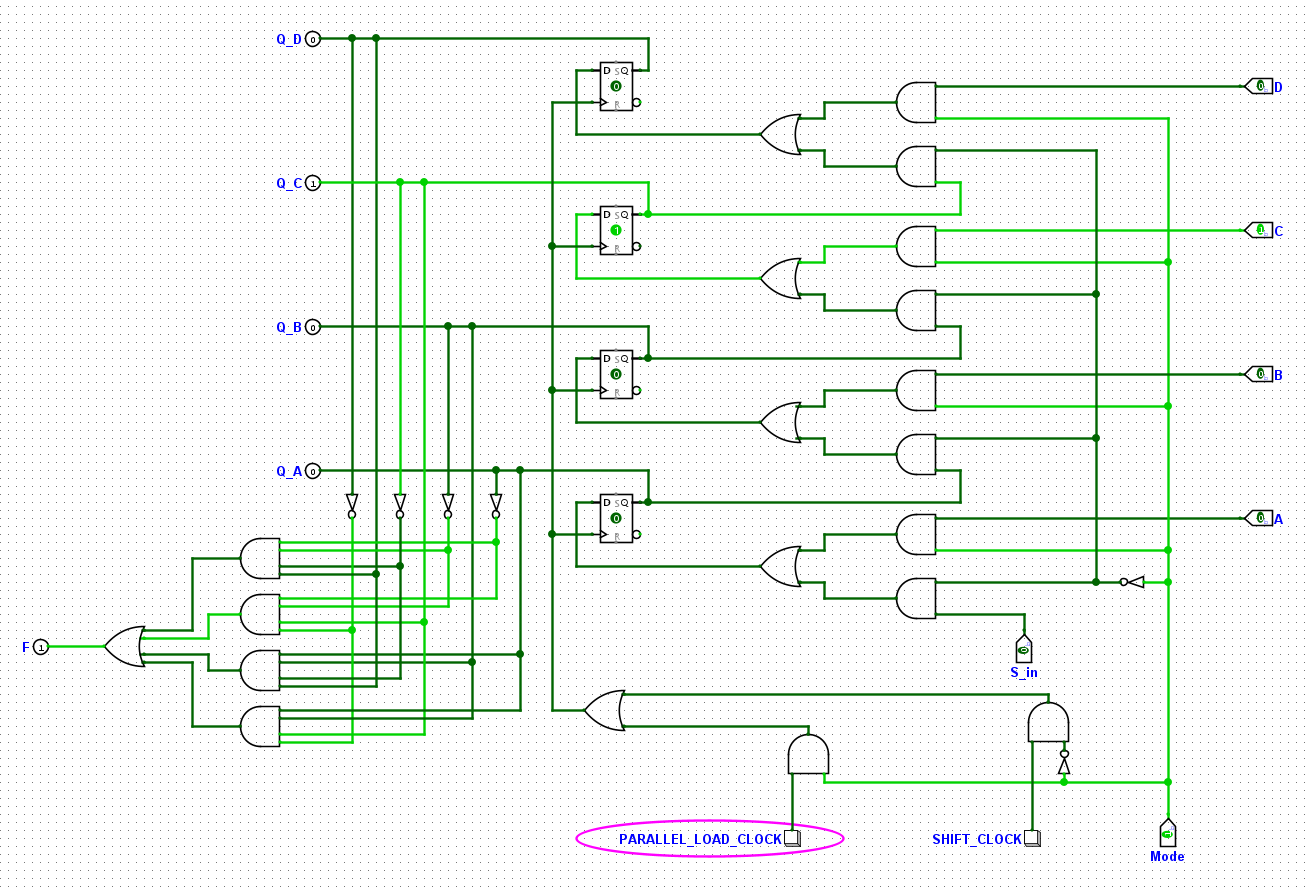
\includegraphics[width=\textwidth]{Screenshot 2026-08-09 171215.png}
		\caption{رشته 0100}
	\end{subfigure}
	
	\vspace{1em}
	
	\begin{subfigure}[b]{0.48\textwidth}
		\centering
		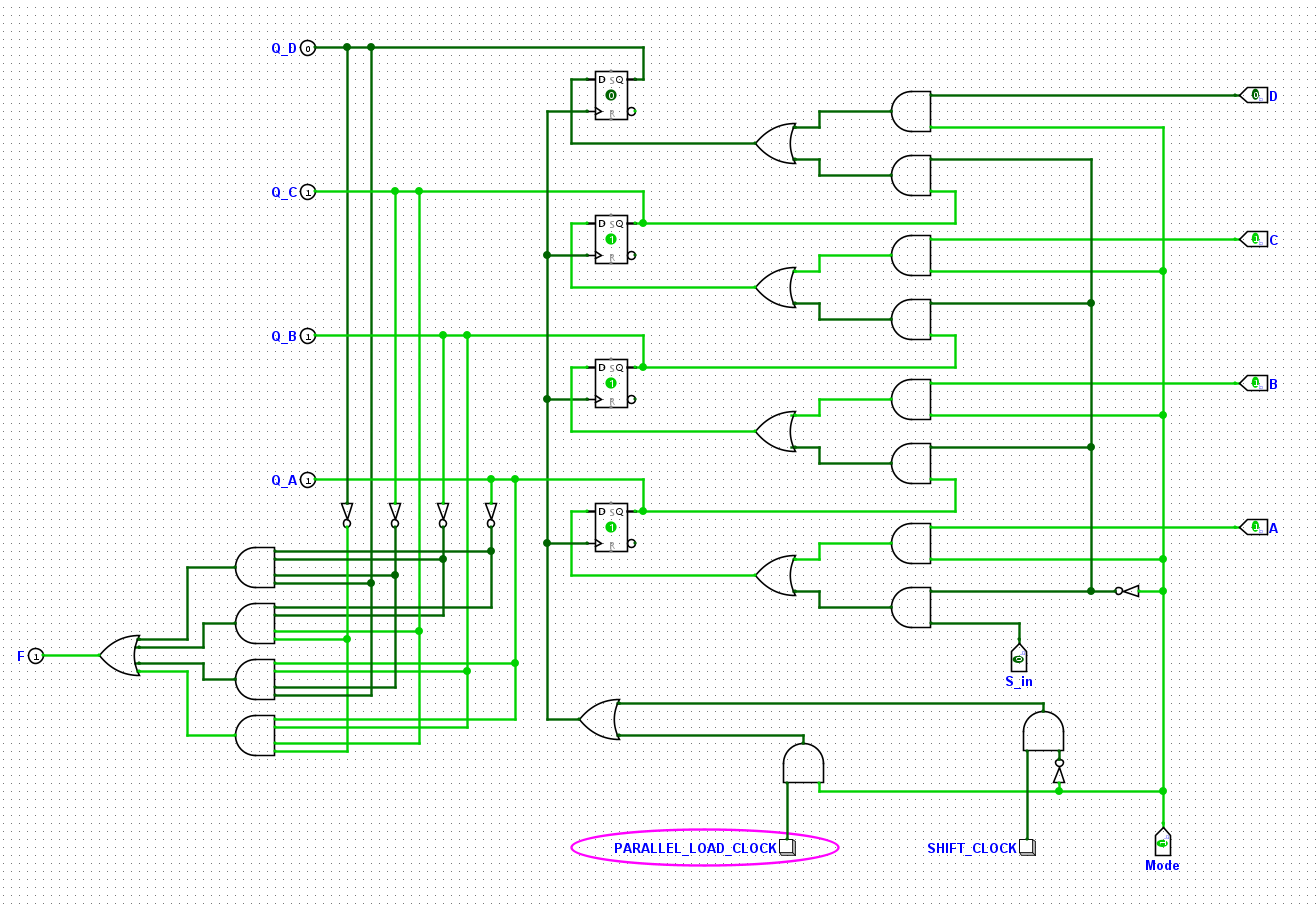
\includegraphics[width=\textwidth]{Screenshot 2026-08-09 171232.png}
		\caption{رشته 0111}
	\end{subfigure}
	\hfill
	\begin{subfigure}[b]{0.48\textwidth}
		\centering
		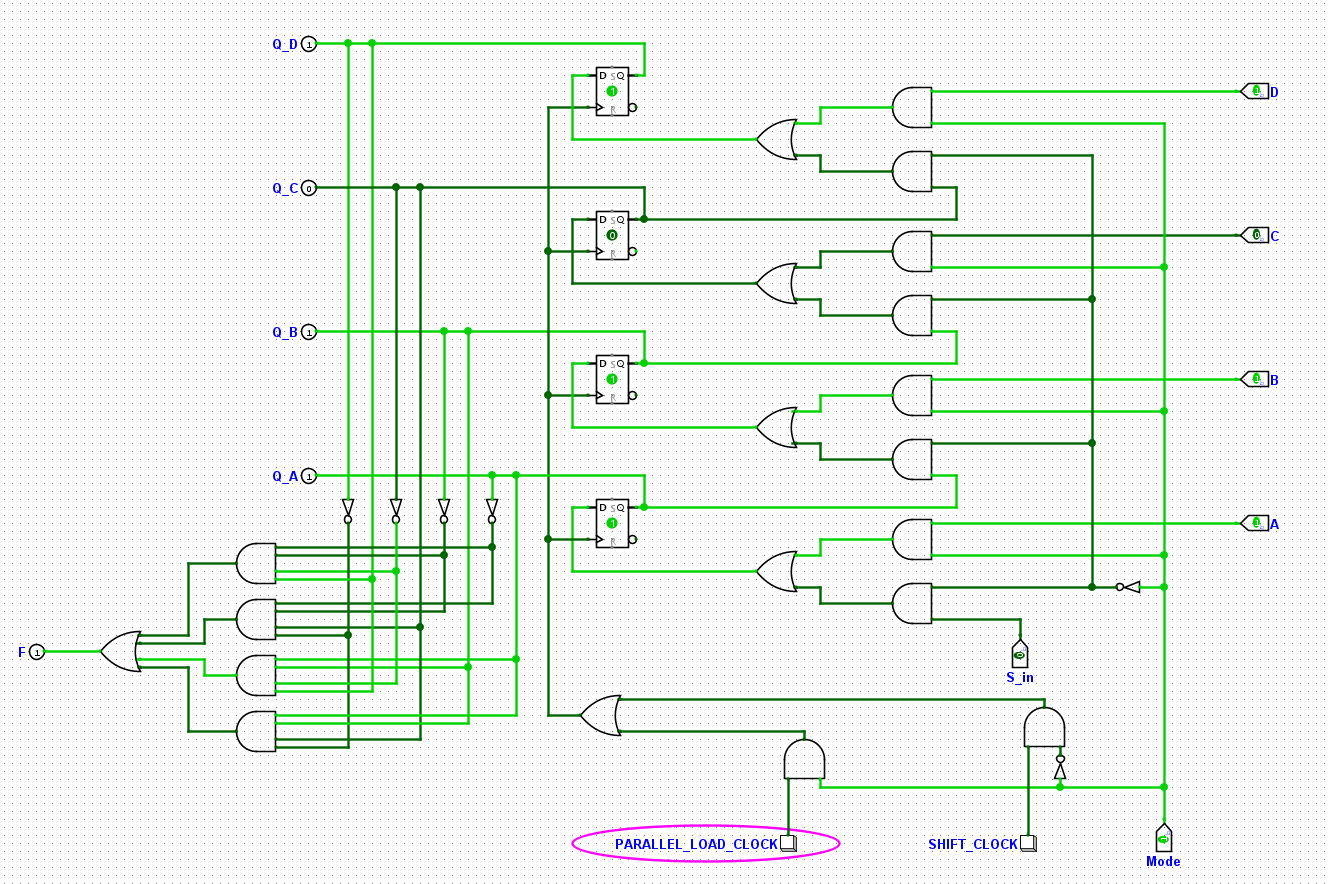
\includegraphics[width=\textwidth]{Screenshot 2026-08-09 171248.png}
		\caption{رشته 1011}
	\end{subfigure}
	
	\caption{نمایش تشخیص رشته های مد نظر}
\end{figure}

\begin{figure}[htbp]
	\centering
	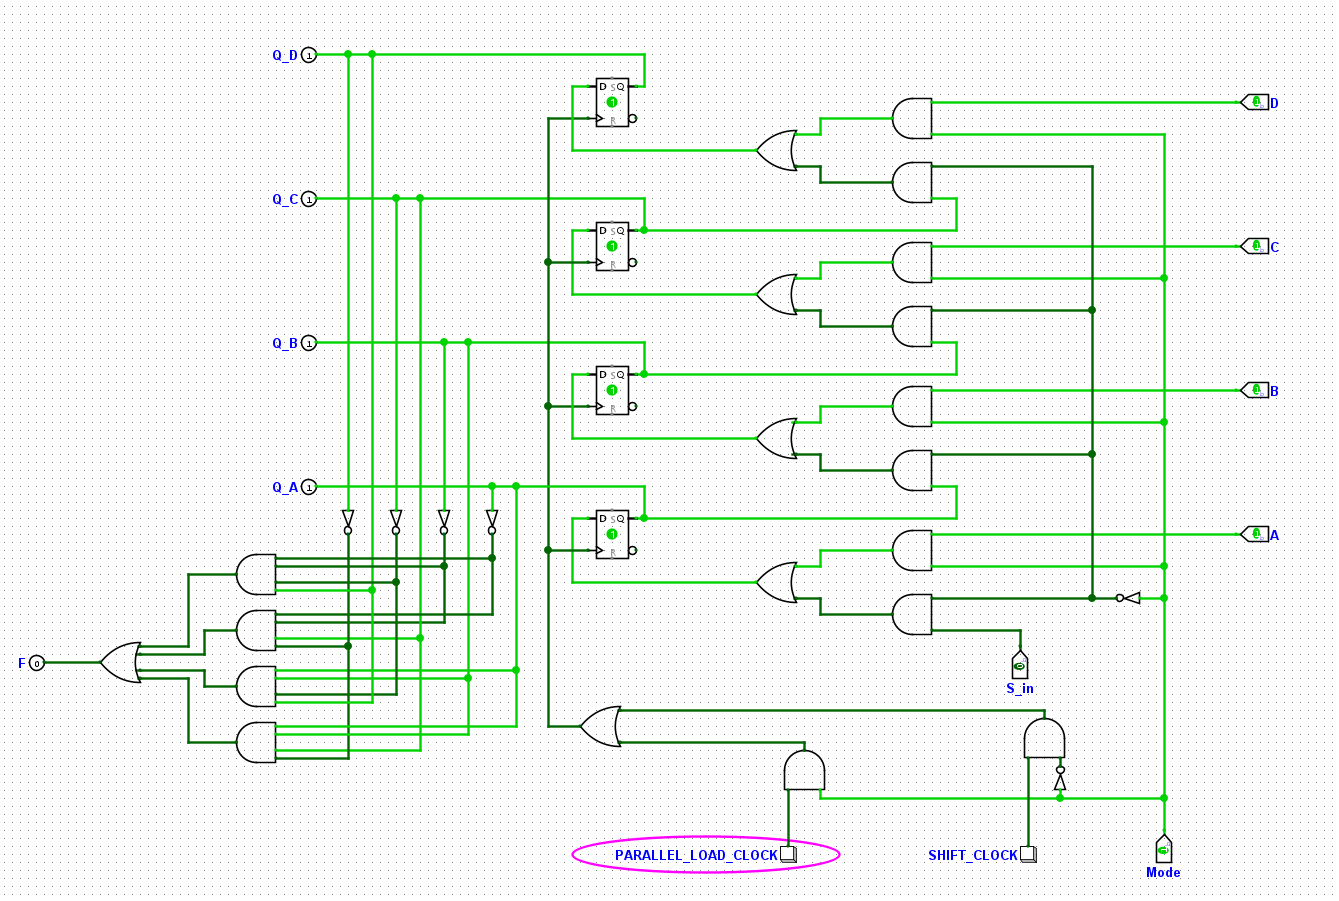
\includegraphics[width=\textwidth]{Screenshot 2026-08-09 171313.png}
	\caption{نمایش خروجی 0 به ازای رشته نامعتبر}
\end{figure}

\clearpage

\section{بررسی \lr{Test Case‌} ها}

در طول آزمایش، صحت عملکرد هر مدار با اعمال چند سناریوی ورودی مشخص و مشاهدهٔ خروجی گام‌به‌گام بررسی شد. مهم‌ترین این سناریوها که تصاویر آن‌ها در بخش‌های قبل ارائه شد، عبارت‌اند از:

\begin{itemize}
    \item \textbf{بارگذاری موازی و شیفت راست (شیفت‌رجیستر یک‌طرفه):} بارگذاری مقدار $1010$ با $Mode=1$ و سپس بررسی گام‌به‌گام ورود $S_{in}$ طی چند تیک کلاک با $Mode=0$ (شکل‌های~\ref{fig:1010-register-initial}، \ref{fig:1010-registered} و \ref{fig:sin-steps-proteus}).
    \item \textbf{شیفت دوطرفه:} بررسی شیفت به چپ در حالت $Mode=1$ (شکل~\ref{fig:twoway-leftshift-example-proteus}) و شیفت به راست در حالت $Mode=0$ (شکل~\ref{fig:twoway_rightshift-example-proteus}) طی چند تیک متوالی، برای اطمینان از عملکرد صحیح هر دو جهت.
    \item \textbf{شیفت‌رجیستر با تراشهٔ 7495:} بارگذاری مقدار $1001$ و سپس شیفت به راست طی سه تیک کلاک متوالی (شکل~\ref{fig:rightshift-example-7459-proteus}).
    \item \textbf{تشخیص رشته:} اعمال رشته‌های معتبر $1000$، $0100$، $0111$ و $1011$ و مشاهدهٔ فعال‌شدن خروجی $F$، در کنار اعمال یک رشتهٔ نامعتبر برای اطمینان از باقی‌ماندن خروجی $F$ در حالت غیرفعال.
\end{itemize}

نتایج این آزمایش‌ها در هر دو محیط Proteus و Logisim یکسان بود که صحت طراحی‌های ارائه‌شده در هر دو پیاده‌سازی را تأیید می‌کند.

\section{نتیجه‌گیری}

در این آزمایش با نحوه کارکرد و پیاده‌سازی شیفت رجیسترها آشنا شدیم. ابتدا با استفاده از فلیپ‌فلاپ‌های D و گیت‌های پایه، یک شیفت رجیستر یک‌طرفه با قابلیت بارگذاری موازی ساختیم و مشاهده کردیم که با کنترل سیگنال $Mode$ می‌توان بین حالت بارگذاری موازی و شیفت سریال جابه‌جا شد. سپس با تغییر ساختار گیت‌های AND ورودی هر فلیپ‌فلاپ، این مدار را به یک شیفت رجیستر دوطرفه تبدیل کردیم که بسته به مقدار $Mode$ قادر به شیفت به راست یا به چپ است.

در ادامه با استفاده از تراشه آماده 7495 نشان دادیم که همان عملکرد شیفت رجیستر با سیم‌کشی بسیار ساده‌تری قابل پیاده‌سازی است، چرا که منطق داخلی بارگذاری و شیفت از پیش در تراشه پیاده شده و کافی است ورودی‌ها، کلاک‌های $SL$ و $SR$ و خروجی‌ها به‌درستی متصل شوند. این مقایسه اهمیت استفاده از تراشه‌های آماده در کاهش پیچیدگی مدار را نشان می‌دهد.

در بخش پایانی نیز با طراحی یک مدار ترکیبی بر پایه جدول درستی و رابطه \lr{SOP}، توانستیم رشته‌های مشخص‌شده (0001، 0010، 1110 و 1101) را در خروجی شیفت رجیستر تشخیص دهیم و صحت عملکرد آن را برای رشته‌های معتبر و نامعتبر بررسی کردیم.

پیاده‌سازی این آزمایش در دو محیط Proteus و Logisim نتایج یکسانی داشت؛ تنها تفاوت قابل‌توجه در بخش استفاده از تراشه 7495 بود، جایی که به‌دلیل نبود این تراشه در Logisim، ناچار به پیاده‌سازی معادلی با دو کلاک مجزا برای دو مود شیفت و بارگذاری شدیم.

\end{document}
